\documentclass[12pt, letterpaper]{report}
\usepackage{XL}  % use my awesome template
\usepackage{pdfsync}
\synctex=1

% \fancyhead[L]{\footnotesize \bfseries Homework 1 \quad \bfseries CS6530 Machine Learning} % set footer
% \fancyfoot[R]{\footnotesize \thepage\ of \pageref{LastPage}} % set footer
\renewcommand{\headrulewidth}{0.0pt} % horizontal line in header
\renewcommand{\footrulewidth}{0.0pt} % horizontal line in footer
\geometry{head=1in, bottom=1in, footskip=25pt} % set margin
\allowdisplaybreaks  % allow cross-page equations


%--------- document starts here -------------------------
\begin{document}

% spacing between equations and text
\setlength{\abovedisplayskip}{-6pt}
\setlength{\belowdisplayskip}{6pt}

\thispagestyle{tpstyle} % set the style of title page
{\centering
\vspace*{3.5in}  % force some space
\textbf{\Huge Computational Fluid Dynamics (CFD) with General Equation Mesh Solver (GEMS)}\vspace{10pt}

\textbf{\Large by Xuxiao Li}\vspace{10pt}

\textit{\large May 3, 2020}
\vspace{8pt}
\centerline{\rule{0.5\linewidth}{0.5pt}}
\vspace{8pt}
\clearpage
\pagenumbering{arabic}  % Number page from the next page
}

\tableofcontents{}

\chapter*{Prologue} \pagestyle{plain} In this document, I will cover multiple topics on both the
theoretical and practical aspects of computational fluid dynamics (CFD). With such a rich range of
contents in CFD, I will only focus on certain methods that I am specialized in, while general
concepts will only be briefly discussed. The major method discussed in this document will be the Finite
Volume Method (FVM). FVM is a somewhat ``old school'' method compared to the more recent and
advanced variants of the Finite Element Method (FEM). However, each method has its own advantages
and disadvantages when applied to specific problems. FVM served for a long period of time as the
workhorse in solving the fluid mechanics problems, while FEM was born to solve solid mechanics
problems. This is a big gap between the ``fluid'' and the ``solid'' community. The trend is
to merge the merits from both methods (e.g., discontinuous Galerkin), but that is still an ongoing
research topic and indeed, old habits die hard.  \paraspace

Within the ``fluid'' community, there is a division between those studying compressible flow
problems and those studying incompressible flow problems. Accordingly, the CFD methods can be
divided into the density-based methods (suitable for compressible flow) and pressure-based methods
(suitable for incompressible flow). The major difference here is that the fluid velocity in
compressible flow is typically large and comparable to the sound speed, while fluid velocity is
relative small for incompressible flows (small Mach number). This gap has already been filled
through years of efforts.  Specifically, density-based methods can also solve incompressible flow
problems using the preconditioning technique, which gives a unified framework for solving fluid
dynamics problems. This approach will be the focus of this document.  \paraspace

In the 80's, there were several pioneers who contributed significantly to the preconditioning
methods, e.g., Eli Turkel, Bram Van Leer, and Charles Merckle. This document will be focused on
Merckle's preconditioning system, and in fact, the practical part of the document is made based on
one of the in-house codes developed at Merckle's research group. The in-house code is named as the
General Equation Mesh Solver (GEMS) whose main creator is Dr. Ding Li. He worked as a research
associate with Prof. Merckle, initially at the University of Tennessee, and later at Purdue
University. Dr. Li embarked on the development of GEMS about early 1999. In 2002, the version 1.0 is
completed. In 2005, he has added the Maxwell equation into GEMS and also refined multiple features
to improve the generality of the code. In a paper Dr. Li published in 2006, he demonstrated the
capability of GEMS with impressing results.
\paraspace

I feel obliged to mention how I can have the access to the GEMS code. During the time Dr. Ding Li
was at Purdue university, there was a PhD student named Shaoyi Wen who worked with Dr. Li. Shaoyi
was then advised by Prof. Yung Shin whose research group had some collaborations with Prof.
Merckle's group. Shaoyi modified GEMS code for his needs with the help of Dr. Li and published a
paper in 2010 using GEMS to solve thermal-fluid problems in direct laser deposition processes.
Thereafter, the GEMS code seemed to be made available to Prof. Shin's group. Before Shaoyi graduated
from Shin's group, he passed the GEMS code to another PhD student at Shin's group, Wenda Tan. At
this time, Dr. Li has left Purdue (I actually don't know where he went). Wenda has never made
acquaintance with Dr. Li. However, he managed to exploit the GEMS code and have three papers
published in 2013, 2014 and 2015 with it. In these papers, Wenda simulated the laser keyhole welding
processes, and with GEMS, his model incorporated multiple physics and has high fidelity. In 2015,
Wenda ceremoniously graduated from Purdue and became an assistant professor at the University of
Utah. In the fall of 2015, I was registered as a PhD student at the University of Utah and I was
advised by Wenda (Dr. Tan) since then. Therefore, I have the privilege to study the GEMS code and
apply it for my PhD research. I have been exploring the GEMS code since 2017 and still learn new
things about it today. So far I only touched upon the ``basic'' functions in GEMS which is to solve
the basic equations: mass, momentum, energy, and species conservation equations. The unexplored part
is: turbulence modeling and incorporation of Maxwell equations. In the definitive version of the
GEMS, all the equations could be solved and can be customized such that multiple sets of equations
can be assigned to different partitions of the domain. In this document, I will focus on the
``basic'' package which I feel the most comfortable with.  \paraspace

The philosophy of this document will be that more focus is put on the theoretical side. By that I
do not mean that I will linger on derivations of equations, as ``computational'' fluid dynamics
should emphasize on {\bf data structure} and {\bf algorithm} and not on mathematical
reasoning. However, I will not go into details such as ``this subroutine does this'', or ``this
variable is used for this'', or ``how do I output such information''. Instead, I will try to {\bf
speak out} what the code is trying to do, why it should be doing this, and how certain things are
done. With this global picture, you should be able to ``code it up'' by any language, any way you
want. In situations where practical guide is necessary, I will try to separate it by distinct
sections.

\chapter{Mesh} \label{c1}

\section{Definition of Basic Mesh} \label{c1s1}

The mesh describes the data structure of carrying out CFD simulations. Mesh is a discretization of a
calculation domain (a physical domain in which CFD simulations is conducted). For example, we have a
two-dimensional rectangle in which we want to carry out CFD simulations, as shown in Fig.
\ref{figmesh1}a. An exemplary mesh is shown in Fig. \ref{figmesh1}b. The rectangle has a width of
2 of a height of 1. The boundary conditions are defined as follows. The left and right edge form
boundary condition batch 1, the top edge is boundary condition batch 2, and the bottom edge is
boundary batch 3. 

\begin{figure}[H]
   \centering
   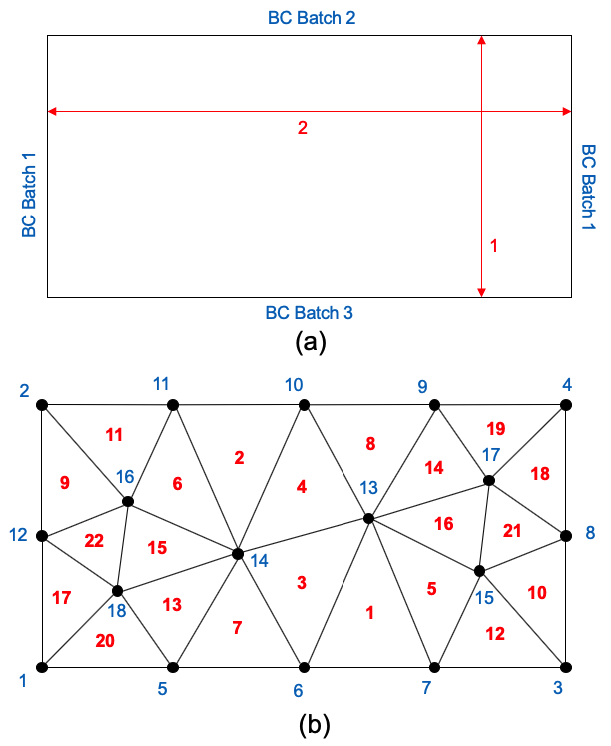
\includegraphics[height=4in]{Mesh1.png}
   \caption{Illustration of mesh. (a) Definition of the calculation domain. (b) A discretization of
   the calculation domain (mesh).}
   \label{figmesh1}
\end{figure}

Several notes on defining the calculation domain. First, the dimensions are be scaled up or down
when simulating a particular problem. That is, the numbers of 1 and 2 can mean ``meter'' or
``micrometer'' depending on the specific problem. No need to specify units here. Second, the
boundary conditions must be carefully stated. We need to first think about how many distinct BC's we
want to define. Then we assign each distinct BC (BC batch) to a segment of the domain boundary. Here,
we have three unique BC's. Each of them is assigned with a certain segment of the domain boundary.
\paraspace

After the calculation domain is defined. We seed the domain with a set of points (black circles in
Fig. \ref{figmesh1}b) in the domain, referred to as the ``{\bf nodes}''. The nodes are indexed by
the blue numbers. We have 18 nodes in the domain. Next, we connect the nodes to form a
``tessellation'' of the domain. Here we use all triangles. In general, there is a large flexibility
of the tessellation. You can use triangles, polygons, or their mixture in two-dimension. In
three-dimension, there are the tetrahedral, pyramid, prism, and hexagon, or their mixture (called
hybrid mesh). This flexibility is incorporated in the GEMS code, therefore the name ``General
Equation Mesh Solver''.  Now with the tessellation, we divide the domain into triangular
``elements'', from which the name ``Finite Element Method'' is originated. However, we will only
focus on the Finite Volume Method in this document, and the elements will be referred to as the
``{\bf cells}''. We have 22 cells in the domain and they are indexed with the red numbers. It should
be mentioned that the indexing order of the nodes and cells does not matter in the definition of the mesh.
\paraspace

Now we can define the ``{\bf cell-node connectivity}'' by associating cells with its corresponding
nodes. For example:
\begin{verbatim}
   cell 1 ---> node 6, 7, 13
   cell 2 ---> node 11, 10, 14
   ...
\end{verbatim}
With that, let's design the following data structures \verb+cell+ and \verb+node+ to better
represent this information. For \verb+node+, we have (in Fortran):

\begin{lstlisting}{language=[90]Fortran}
   type node
      real :: xyz(ndim)
   end type node
\end{lstlisting}

where \verb+ndim+ is the number of dimensions and \verb+xyz+ is the coordinate of the node. We will
need to have an array of nodes \verb+nodes(:)+ to store all the information about nodes. For cells,
we have the following data type:

\begin{lstlisting}{language=[90]Fortran}
   type cell
      real :: centp(ndim)
      integer, pointer :: c2n(:)
   end type cell
\end{lstlisting}

where \verb+centp+ is the centroid of the cell and \verb+c2n+ is the node indices associated with
this cell. Note that we can calculate the centroid of the cell based on the nodal coordinates
associated with the cell. We will also need an array of cells \verb+cells(:)+ to store all the
information about cells. Now we have introduced two important data types \verb+node+ and
\verb+cell+. Each of these data types can have more attributes which we will build on later.
\paraspace

Now we still need to add the last part of the mesh definition, the boundary conditions. To define
the boundary conditions of the mesh, we have to introduce another important concept, ``{\bf
faces}''. Faces are the edges (or facets in 3D) that form the boundary of a cell. There are three
faces per one triangle cell, and six faces per one hexagon cell (in 3D), etc. Faces that are shared between
two cells are defined as {\bf interior faces}. Faces that are only belong to a single cell are
defined as {\bf boundary faces}. Faces can be distinguished by a set of nodes, which brings about
the ``face-node'' connectivity. We will discuss in further details about faces in the next section.
For now, we use face to define the boundary conditions as follows:
\begin{verbatim}
   BC batch 1 ---> 4 faces: (1, 12), (2, 12), (3, 6), (4, 8)
   BC batch 2 ---> 4 faces: (2, 11), (11, 10), (10, 9), (9, 4)
   BC batch 3 ---> 4 faces: (1, 5), (5, 6), (6, 7), (7, 3)
\end{verbatim}
That is, we use the boundary faces (shown as node sets above) to define the segments of boundaries.
Each set of faces represents a unique BC. It is convenient to create a data type for the BC's:

\begin{lstlisting}{language=[90]Fortran}
   type bc_type
      integer :: label
      integer :: igrp
      integer :: itype
   end type bc_type
\end{lstlisting}

Here, \verb+label+ is a distinct integer to indicate the batch of BC. \verb+igrp+ indicates which
``group'' of BC it is. In GEMS, there are 6 groups of BC's: 

\begin{itemize}
   \item Group 1, Inlet
   \item Group 2, Outlet
   \item Group 3, Farfield
   \item Group 4, Wall
   \item Group 5, Geometric (e.g., symmetric, periodic)
   \item Group 6, MHD (for Maxwell equations)
\end{itemize}

Each group of BC can have sub-categories (types) which is saved in the attribute \verb+itype+.
Again, we need an array of BC's \verb+bc(:)+ to store all the information. Apparently, the
association between BC and faces should be defined based on the face lists of each batch of BC,
which will be discussed in the next section.
\paraspace

So far, we have introduced the complete information to define a mesh, summarized as follows:

\begin{enumerate}
   \item Nodal coordinates.
   \item Cell-node connectivity.
   \item Face list in each BC batch.
\end{enumerate}

We emphasize this contains the complete information of a mesh. We refer this piece of information as
the ``basic mesh'' or the finite element mesh. The information is complete but is not organized in a
way convenient for finite volume method. As we will see, additional data types can be constructed
based on the basic mesh and be used to facilitate finite-volume computation. 
\paraspace

\clearpage
\section{Finite Volume Mesh} \label{c1s2}

We establish the data type \verb+face+ from the basic mesh to form the ``finite volume mesh''. The
\verb+face+ type has much more emphasis in the finite volume method as the fluxes on the faces need
to be computed. On the opposite side, the finite element method emphasize on the data type
\verb+node+. The \verb+face+ type is defined as:

\begin{lstlisting}{language=[90]Fortran}
   type face
      integer :: itype
      type(cell), pointer :: left_cell
      type(cell), pointer :: right_cell
      integer, pointer :: f2n(:)
      real :: centp(ndim)
   end type face
\end{lstlisting}

Here, \verb+itype+ defines the type of the face which we will elaborate later. The pointers
\verb+left_cell+ and \verb+right_cell+ refers to the two cells that share this face. This is
referred to as the {\bf face-cell connectivity}. The pointer \verb+f2n(:)+, like \verb+c2n(:)+, is
the {\bf face-node connectivity}, which refers to the set of nodes that defines the face. At last,
the center of the face \verb+centp+ can be calculated based on the nodal coordinates which can be
found through \verb+f2n(:)+. The \verb+face+ type constructed based on Fig. \ref{figmesh1}b is
shown in Fig. \ref{figmesh2}. The faces are indexed with the green number and there are 39 faces in
the calculation domain.

\begin{figure}[H]
   \centering
   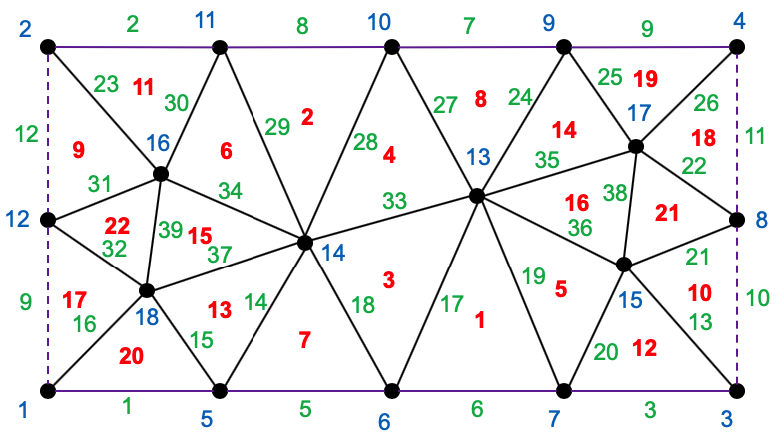
\includegraphics[height=3in]{Mesh2.png}
   \caption{Construction of faces to make the finite volume mesh.}
   \label{figmesh2}
\end{figure}
\paraspace

How to collect all the face information from the basic mesh? The face information can be found from
the cell-node connectivity. For example:

\begin{verbatim}
   cell 1 ---> node 6, 7, 13, we can find:
      face 1 --> node 6, 7
      face 2 --> node 7, 13
      face 3 --> node 13, 6
   cell 2 ---> node 11, 10, 14, we can find:
      face 4 --> node 11, 10
      ...
\end{verbatim}

By doing so we obtain an array of faces, \verb+faces(:)+. Two points need to be noted. First, the
face-node connectivity is contained in the cell-node connectivity, but we still need to know which
nodes in a cell can form a face. If all cells are triangles, any combination of the three nodes of
the cell will form a face. But for quadrilaterals and 3D cells, a set of rules need to be
pre-defined to help extracting the face-node connectivity.  The second note is, faces identified
this way will be double-counted. We need to delete the repeating faces. This can be done by checking
whether the face-node connectivity \verb+f2n+ is repeating. In doing so, every time we find a
repeating face, it means two cells share the same face.  Therefore, the \verb+left_cell+ and the
\verb+right_cell+ can be found. We note that the ``left'' and ``right'' do not mean the literal
directions. In practice, we always make the cell with the smaller index (red number in Fig.
\ref{figmesh2}) to be the left cell and the other cell to be the right cell.
\paraspace

There are some faces that are only belong to a single cell. These faces are referred to as the
``{\bf boundary faces}'' (face 1 - 12 in Fig. \ref{figmesh2}). Boundary faces are regarded as
special faces and we will make them to be at the front of \verb+faces(:)+ by {\bf swapping faces} in the
face array. We assign the only cell
that a boundary face is associated to be the {\bf left cell} of the boundary face. That is, the
boundary faces only have \verb+left_cell+ which is the interior cell, for now.
\paraspace

In CFD computation, it is required that every face be associated with two cells, including the
boundary faces. Therefore, we need to create a ``{\bf ghost cell}'' as the right cell for the
boundary faces. Ghost is an overused word (but I still sometimes use it). The ghost cell is
alternatively referred to as the ``{\bf boundary cell}''. To create the ghost cells, we can simply
mirror the interior cell with respect to the boundary face. However, there is one exception, the
periodic boundary condition. For periodic BC, we need to translate the same cell ``on the other
side'' to form the ghost cell. To illustrate, the boundary faces are marked purple in Fig.
\ref{figmesh2}. We let BC batch 1 to be the periodic BC, and the periodic boundary faces are marked
as dashed purple. To create the boundary cells, we can mirror cell 11, 2, 8, 9, 20, 7, 1, and 12 for
face 2, 8, 7, 9, 1, 5, 6,  3, respectively. For periodic boundary cells, we need to translate cell
9, 17, 18, 10 for face 11, 10, 12, 9, respectively. This indicates that the periodic boundary faces
must ``match'', otherwise, the mesh is ill-defined for the periodic BC. The periodic boundary faces
are special boundary faces. We will move these faces to the end of the boundary faces. That is,
\verb+face(1)+ to \verb+face(12)+ are the boundary faces, and \verb+face(9)+ to \verb+face(12)+ are
reserved for periodic boundary faces.  We will dedicate an entire section to periodic BC later.
\paraspace

One last note about face types. The interior faces (black solid line in Fig. \ref{figmesh2}) has
\verb+itype = 0+. The boundary faces has a positive \verb+itype+ which equals to the index in
\verb+bc(:)+ that the boundary face is associated with. For example, we have 3 batches of BC's, and
we create an array \verb+bc(:)+ with a length of 3. Each element in \verb+bc+ corresponds to one
specific BC batch. Say, batch 1 corresponds to \verb+bc(3)+. Then the \verb+itype+ for face 9, 10, 11,
12 will be equal to 3. There can be other \verb+itypes+ which we shall discuss later.
\paraspace

To summarize, the finite volume mesh consists of the following information:
\begin{enumerate}
   \item Nodal coordinates.
   \item Cell-node connectivity.
   \item Face types, face-cell connectivity and face-node connectivity.
\end{enumerate}
Notice that the information about BC's can be fully described by the \verb+bc(:)+ array and the
\verb+itype+ in \verb+face+.
\paraspace

\clearpage
\section{Partitioning of Mesh} \label{c1s3}

Now we have got a finite volume mesh, with three essential data types, \verb+node+, \verb+cell+, and
\verb+face+. It is no problem to plug this mesh into some CFD code. However, today's computation
lives in a parallel world. Any practical CFD code must enable parallel computing. GEMS uses MPI
for parallel computing. In MPI, the finite volume mesh is decomposed into partitions. Each partition
is assigned to one ``core'' (or one CPU, one ``processing element'', any way you want to call it).
Each core only has information about its own partition of the entire domain and has no idea of what the
entire domain is like. Such a partitioning is shown in Fig. \ref{figmesh3}.

\begin{figure}[H]
   \centering
   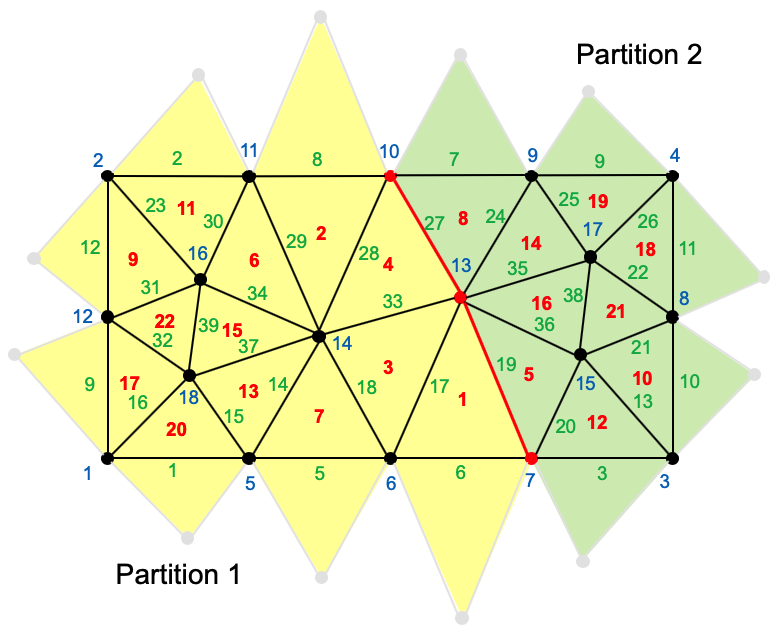
\includegraphics[height=4in]{Mesh3.png}
   \caption{Partitioning of calculation domain}
   \label{figmesh3}
\end{figure}

Here the contour formed by the solid black line is the calculation domain, including the nodes
(indexed by blue), cells (indexed by red) and faces (indexed by green). We also show the ghost cells
(boundary cells) marked by the gray lines. It is noted that the ghost cells can be entirely derived
from the boundary faces and need not be store prior to CFD simulation. Based on this configuration,
we partition the domain into two partitions. First, we identify which {\bf cells} belong to which
partition. Then the nodes and faces shared by cells from both partitions can be identified (marked
by red). These delineates the {\bf interface} of the partitions. The nodes, cells, and faces belong
to partition 1 is shadowed by yellow and those belong to partition 2 is shadowed by green.
\paraspace

Now we split the domain into two partitions as shown in Fig. \ref{figmesh4}. Take partition 1 for
example, the nodes, cells, and faces all need to be re-indexed as partition 1 does not have any
information about partition 2. The re-indexed numbers are shown by the corresponding blue, red and
green numbers. For partition 1, to establish the ``communication'' with the external world (which
means partition 2 in this case), we identify all the cells (including ghost cells) in partition 2
that shared nodes with partition 1. Those are the orange-shaded cells indexed from 1 - 7. This means
there are 7 cells we need to create in partition 1 as ``containers'' to receive the information from
partition 2. Same for partition 2, we need to create 6 ``container'' cells to receive information
from partition 1. From a global point of view (Fig. \ref{figmesh3}), the container cells
(orange-shaded cells in Fig. \ref{figmesh4}) for both partitions can be identified. Then, we can
correspondingly mark in each partitions the cells that need to be ``sent'' out to the external
world (the sky-blue shaded cells in Fig. \ref{figmesh4}). Note that the ``sending cells'' and the
``receiving cells'' must match. That is, the receiving cells in partition 1 (orange) must be match
the sending cells in partition 2 (sky-blue), and vice versa.

\begin{figure}[H]
   \centering
   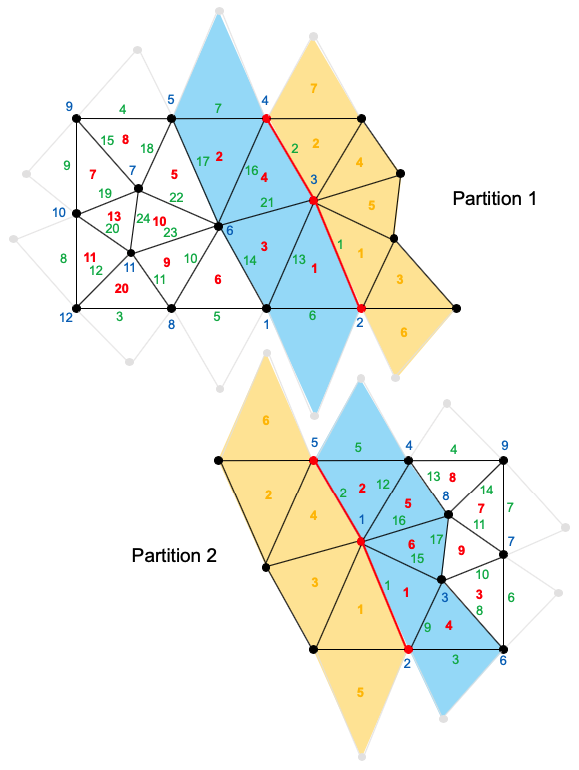
\includegraphics[height=6in]{Mesh4.png}
   \caption{Splitting of the domain and re-indexing.}
   \label{figmesh4}
\end{figure}
\paraspace

To represent the data structure for communication among partitions, in GEMS, the data type
\verb+itf+ (standing for ``interface'') is created: 

\begin{lstlisting}{language=[90]Fortran}
   type itf
      integer :: nn
      integer, pointer :: np(:), nnp(:)
      type(cell), pointer :: pcell(:) 
   end itf
\end{lstlisting}

where \verb+nn+ is the number of partitions from which the current partition receives data; \verb+np+
and \verb+nnp+ are arrays with a length of \verb+nn+. \verb+np+ stores the id of the partitions from
which the current partition receives data, and \verb+nnp+ stores the number of cells to receive from
each partition. Finally, \verb+pcell+ is the array of ``container'' cells to store the received
data. \verb+pcell(:)+ should have a length of \verb+sum(nnp)+. It should be noted that the
\verb+pcell(:)+ array needs to be {\bf allocated} as it is ghost cells that do not exist in the
physical domain of partition 1. 
\paraspace

So far, the attributes of \verb+itf+ are only relative to receiving (orange-shaded cells in Fig. \ref{figmesh4}). We need to add similar attributes for sending:

\begin{lstlisting}{language=[90]Fortran}
   type itf
      ...
      integer :: nc
      integer :: cp(:), ncp(:)
      type(neighbour_cell), pointer :: scell(:)
   end type itf
\end{lstlisting}

Here \verb+nc+ is the number to partitions to which the current partition needs to send data;
\verb+cp+ is the id's of partitions to which the current partition sends data and \verb+ncp+ is the
number of cells to send to each partition in \verb+cp+. The array \verb+scell(:)+ points to the
cells in the current partition whose information will be sent to external partitions. Notice that
instead of using \verb+type(cell)+, we invented a new data type \verb+neighbour_cell+ for
\verb+scell(:)+. This data type is a {\bf nested type} for the type \verb+cell+:

\begin{lstlisting}{language=[90]Fortran}
   type neighbour_cell
      type(cell), pointer :: to_cell
   end type neighbour_cell
\end{lstlisting}

There is nothing in the type \verb+neighbour_cell+ but a \verb+cell+ pointer. This nested structure
is adopted in GEMS to represent that the cell pointer {\bf needs not be allocated}. Rather, it is
merely a reference to cells already allocated.
\paraspace

How can we construct such data type \verb+itf+? It must start from the global domain (Fig.
\ref{figmesh3}). First we identify the container cells for each partition (1 \& 2). Then we can
identify the sending cells in partition 1 based on the container cell in partition 2, and we record
the cell id's and boundary face id's (for boundary cells to send). Same for partition 2. For
container cells, they don't yet exist in each partition. Therefore, (for example, in partition 1), we simply
allocate 7 ``empty'' cells. The empty cells will be fulfilled once the data is received from
partition 2.
\paraspace

Although the container cells are empty, the cell-node and cell-face connectivity between the
container cells and the nodes and faces needs to be identified. Take partition 1 for example, for
cell-node connectivity, we need to record in each container cell which node index in partition 1 it
is associated with. Note, only record those nodes in partition 1, so we have 2 nodes for
\verb+pcell(1:2)+ and only 1 node for \verb+pcell(3:7)+. For face-cell connectivity, we need to
associate the \verb+right_cell+ of \verb+faces(1:2)+ with \verb+pcell(1:2)+ for partition 1. For
partition 2, we associate the \verb+right_cell+ of \verb+faces(1:2)+ with \verb+pcell(1)+ and
\verb+pcell(4)+. The \verb+left_cell+ will be assigned to the other cell which is interior cell. It
should be mentioned that the \verb+left_cell+ of a face always belong to the interior of the domain.
\paraspace

The indexing convention for the partitioning is as follows. We first index interior cells for
\verb+pcell+ and then the boundary cells. Same for the \verb+scell(:)+. Note, the indexing of
\verb+scell(:)+ and \verb+pcell(:)+ must match across partitions. The faces that has a
\verb+right_cell+ as a container cell are referred to as the ``{\bf partitioning faces}'' and are
considered as another type of special faces. A special (large) number is reserved for the
\verb+itype+ of the partitioning faces, 19621011. The partitioning faces are indexed from very
beginning of the \verb+faces+ array (by proper face swapping). Therefore, we have a rather complex
rule for face indexing (take partition 1 as example):

\begin{enumerate}
   \item Index partitioning faces (face 1 \& 2), \verb+itype = 19621011+
   \item Index boundary faces that are not periodic boundaries (face 3 - 7), \verb+itype = + positive
      number (from one to the number of BC's)
   \item Index periodic boundary faces (face 8 \& 9), \verb+itype = + the number for periodic BC
   \item Index interior faces (face 10 - 23) , \verb+itype = 0+
\end{enumerate}

Also, we record the number of partitioning faces in the type \verb+itf+ by adding the variable
\verb+nitf+:

\begin{lstlisting}{language=[90]Fortran}
   type itf
      ...
      integer :: nitf
   end type itf
\end{lstlisting}
\paraspace

With the mesh partitioning, we will generate separate mesh files for each partition. Let us now
summarize the information contained in each mesh file:

\begin{enumerate}
   \item Nodal coordinates for current partition
   \item Cell-node connectivity for current partition
   \item Face-cell connectivity, face-node connectivity as well as face type for current partition
   \item Sending information: No. of sending-to partitions, No. of total sending cells. For each
      sending-to partition,
      \begin{enumerate}
         \item sending-to partition id, No. of to-be-sent interior cells, No. of to-be-sent boundary cells
         \item for to-be-sent interior cells, store those cell id
         \item for to-be-sent boundary cells, store those boundary face id
      \end{enumerate}
   \item Receiving information: No. of receive-from partitions, No. of total receiving (container)
      cells. For each receive-from partition, 
      \begin{enumerate}
         \item receive-from partition id, No. of container cells to receive from this partition
         \item for each container cell, record the node shared between container cell and the
            current partition
      \end{enumerate}
\end{enumerate}
\paraspace

\clearpage
\section{Periodic Boundary Condition} \label{c1s4}

The treatment of periodic BC deserves a separate section to describe. The difficulty in treating
periodic BC arises when information in the boundary cells for periodic BC cannot be directly
obtained from the left cell of the boundary face (i.e., mirroring). Rather, we need to find the left
cell of the matching boundary face ``on the other side''. Moreover, when the domain is partitioned,
the matching face may not even exist in the current partition, and communication must be established
specially for treating periodic BC.
\paraspace

To better illustrate the treatment of periodic BC, we modified the original definition of BC's in
Fig. \ref{figmesh1}. As shown in Fig. \ref{figmesh5}a, we define only two batches of BC's and both of them are
assigned to be periodic BC's. Each batch consists of a pair of walls. The corresponding mesh (before
partition) is shown in Fig. \ref{figmesh5}b. We emphasize again that boundary faces in the mesh for periodic BC
must ``match'', i.e., sharing the exact same nodal coordinates in all directions excluding the
periodic direction. Otherwise, the face meshing is ill-defined for the periodic BC.

\begin{figure}[H]
   \centering
   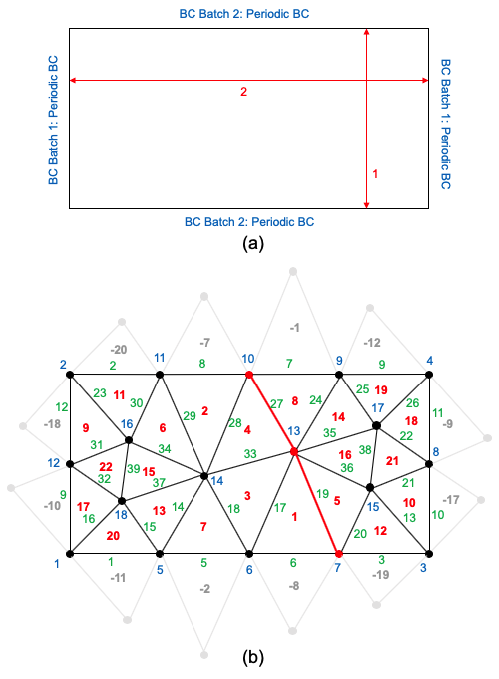
\includegraphics[height=5in]{Mesh5.png}
   \caption{Re-define the boundary conditions. (a) Set two pairs of walls as 2 batches of periodic
   BC. (b) The mesh corresponding to the setup in (a).}
   \label{figmesh5}
\end{figure}
\paraspace

In Fig. \ref{figmesh5}b, again, the node, cells, and faces of the global domain are indexed. The
global domain will be partitioned into two parts as separated by the red line like before. The
boundary cells are marked by the gray edges. The first step to construct periodic BC is to find the
``matching cells'' for the boundary cells. This step is shown with the global indices in Fig.
\ref{figmesh5}b. We index the periodic boundary cells by a negative number whose absolute value
matches the global indices of the matching interior cells, as shown in Fig. \ref{figmesh5}b. After
the matching cells are found (globally), we merge the two (or more) batches of periodic BC as one
batch. This is due to the special treatment of periodic BC in GEMS. As long as matching cells are
found, the complete information regarding to all periodic BC's is known. Therefore, they are viewed
as a single package (of BC) in GEMS.  \paraspace

Now, let's illustrate the specific data structure of periodic BC by considering the partitioning
layout shown in Fig. \ref{figmesh6}. Take partition 1 for example, the yellow region is the
physical domain of partition 1 and the orange region is the container cells to receive information
from partition 2, like before. There are 7 container cells, as indexed by the orange numbers. Now,
the periodic boundary cells are considered as a second type of container cells, as indexed by the
purple numbers. There are 8 {\bf periodic container cells} and they are indexed as negative number to
differentiate with the ``partitioning container cells''. It is noted that some of these periodic
container cells needs to be received from partition 2 (-4, -6 and -7), but some of them are actually
just the interior cells
in partition 1 but ``on the other side'' of the boundary faces of -2, -5, -1, -3. GEMS will treat all
the periodic container/boundary cells by communications between partitions, in a unified manner. For
cell -2, -5, -1 and -3, they will be communicated from partition 1 and to partition 1. This is the
difference between communicating partitioning cells and periodic boundary cells. The latter involves
communicating with the partition itself (totally OK in MPI).

\begin{figure}[H]
   \centering
   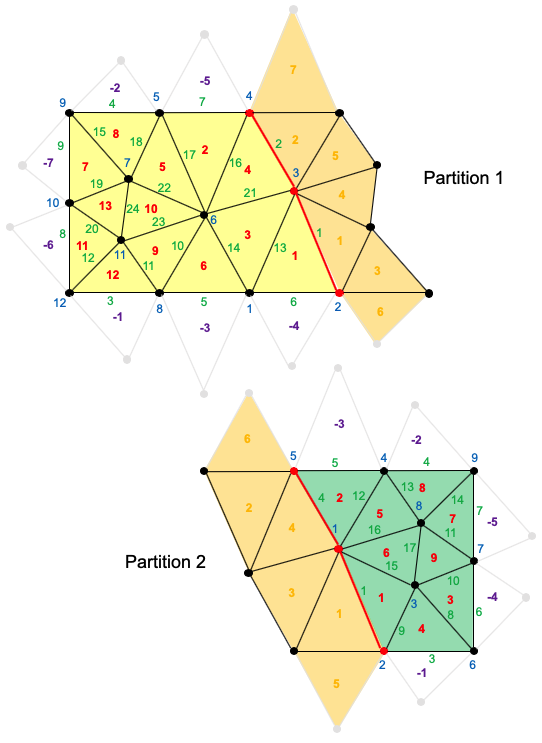
\includegraphics[height=6in]{Mesh6.png}
   \caption{Demonstration of the treatment of periodic BC.}
   \label{figmesh6}
\end{figure}
\paraspace

If we examine on the interior cells in Fig. \ref{figmesh5}b, each interior cell belongs to a
unique partition (separated by the red line). Also, with the matching cell known for each
periodic boundary face, we can know from where the periodic container cells should receive.
The exact same data structure \verb+itf+ as in partitioning communication is used to represent
the communication for periodic BC. \verb+pinterf+ (of the type \verb+itf+) can be constructed in both
partitions in the following way:

\begin{verbatim}
   pinterf of Partition 1:
      2 receiving batches:
      receive-from id ---> 1 (itself) and 2
      No. of container cells ---> 4 (from id = 1) and 3 (from id = 2)
      periodic boundary faces to bear the container cells:
         face 4, 7, 3, 5 for from id = 1
         face 8, 9, 6 for from id = 2

      2 sending batches:
      sending-to id ---> 1 (itself) and 2
      No. of to-be-sent cells ---> 4 (to id = 1) and 3 (to id = 2)
      To-be-sent iterior cell indices:
         cell 8, 2, 6, 11 for to id = 1
         cell 7, 11, 1 for to id = 2
   end pinterf

   pinterf of Partition 2:
      2 receiving batches:
      receive-from id ---> 1 and 2 (itself)
      No. of container cells ---> 3 (from id = 1) and 2 (from id = 2)
      periodic boundary faces to bear the container cells:
         face 4, 5, 3 for from id = 1
         face 6, 7 for from id = 2

      2 sending batches:
      sending-to-id ---> 1 and 2 (itself)
      No. of to-be-sent cells ---> 3 (to id = 1) and 2 (to id = 2)
      To-be-sent iterior cell indices:
         cell 2, 7, 3 for to id = 1
         cell 8, 4 for to id = 2
   end pinterf
\end{verbatim}

In constructing the above data structure, we first identify the container cells in both partitions.
These are ``ghost cells'' to be allocated and are not interior cells in the domain. Then, the
sending cells (interior cells) are determined based on the container cells in each partition. It is
noted that for periodic boundary cells, we do not need the cell-node connectivity as in partitioning
cells. We only need the cell-face connectivity. We associate periodic boundary faces with their
corresponding container cells. Then, the cell-node connectivity of the container cells is equivalent
to the face-node connectivity of the periodic boundary faces. This can be applied to other type of
boundary cells. The cell-node connectivity of boundary cells will always be equivalent to the
face-node connectivity of the corresponding boundary faces.
\paraspace

As a final note, the communication of periodic BC must precede the communication of the
partitioning. This is because we periodic BC communication will first fill in all the boundary
cells, some of which can then be sent out via the partitioning communication.
\paraspace

\clearpage
\section{Practical Guide}
We shall give some practical instructions in the section regarding the generation and use of mesh
files. The action items are summarized by the flow chart shown in Fig. \ref{figmesh7}. 

\begin{figure}[H]
   \centering
   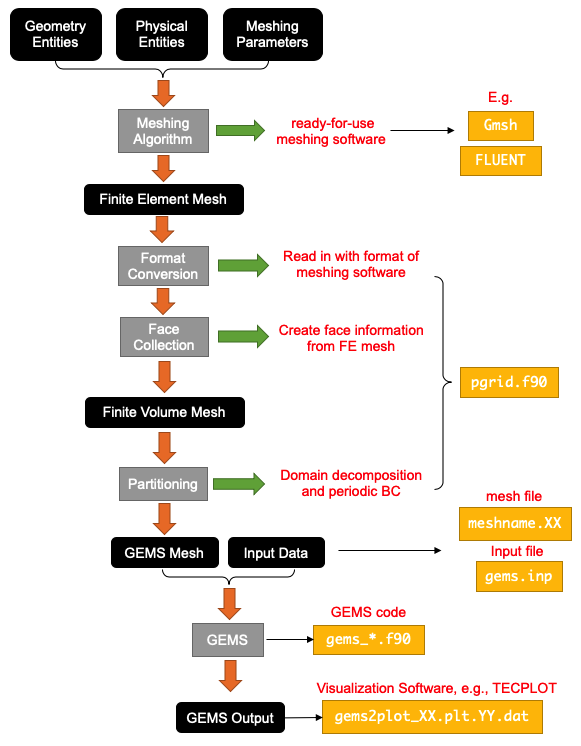
\includegraphics[height=6in]{Mesh7.png}
   \caption{Flow chart of generating and using mesh files.}
   \label{figmesh7}
\end{figure}

The first step is to generate a finite element mesh as described in section \ref{c1s1}. We note that
the mesh file is defined by three components: geometry entities, physical entities, and meshing
parameters. The geometry entities refer to the point, lines, curves, etc. that define the geometry
of the calculation domain. This is analogous to the CAD drawing you use for a design. Second, you
associate the geometry entities with physical entities. For example, the geometry entities in Fig.
\ref{figmesh1}(a) is 4 points, 4 lines and a rectangle. The lines that form the rectangle are
associated with physical entities BC batch 1 (e.g., periodic boundaries), BC batch 2 (e.g., solid
wall) and BC batch 3 (e.g., another solid wall). Finally, the meshing parameters that specify the
way to ``seed'' the domain with nodes are defined. That can be how many nodes should be seeded along
the lines, etc. The geometry entities, physical entities, and meshing parameters are then fed into
the meshing algorithm to generate a finite element mesh like that in Fig. \ref{figmesh1}(b).
\paraspace

The meshing algorithm itself is a totally different science. We simply rely on ready-for-use
toolboxes to generate the finite element mesh, rather than implement the mesh algorithm ourselves.
\verb+Gmsh+ seems to be a good option for doing this, as it gives flexible automation with Gmsh
scripts. However, you still need to learn how to draw points and lines, associated them with physical
entities, as well as control the meshing schemes with meshing parameters. For \verb+Gmsh+, those are
specified in the \verb+.geo+ files, which are inputted into \verb+Gmsh+ to obtain the mesh
(\verb+.msh+) files.
\paraspace

Once we have the FE mesh file, we feed it into the code \verb+pgrid.f90+ which is a part of GEMS
code and functions as a pre-processor to convert a FE mesh to the mesh file GEMS recognizes
(referred to as the GEMS mesh). In \verb+pgrid.f90+, the first task is to read in the FE mesh
generated by other software (e.g. \verb+Gmsh+). Unfortunately, the software usually writes a mesh
file in complicated ways, and different software writes the mesh file differently. \verb+pgrid.f90+
has different interfaces for reading FE mesh files with different format, but mostly of them are
obsolete. For example, the \verb+GAMBIT+ format was used in the past which is generated by
\verb+FLUENT+. But since \verb+FLUENT+ was acquired by \verb+ANSYS+, we have lost the way to
generate \verb+GAMBIT+ files.  As of today, two formats are actively used: (1) Cartesian mesh
format, which is generated without using any software, and (2) SU2 format, which is generated by
\verb+Gmsh+ (choose \verb+SU2+ format when exporting).  \paraspace

The Cartesian mesh format is a simple format and it can be written in the following way (in
FORTRAN, and use a 2D mesh as example):

\begin{lstlisting}{language=[90]Fortran}
   do j=1, Nj
      do i=1, Ni
         write xn(i)
      end do
   end do

   do j=1, Nj
      do i=1, Ni
         write yn(j)
      end do
   end do
\end{lstlisting}

Here \verb+Ni+ and \verb+Nj+ are the number of {\bf nodes} (not cells) along each dimension. \verb+xn(:)+ and
\verb+yn(:)+ are 1D arrays that contains the nodal coordinates along X and Y dimension,
respectively. Besides this, the boundary condition information must be written in a separate file in
the following way:

\begin{lstlisting}{language=[90]Fortran}
   write ndim*2
   write 1,Ni,1,1,0,0,label1
   write 1,Ni,Nj,Nj,0,0,label2
   write 1,1,1,Nj,0,0,label3
   write Ni,Ni,1,Nj,0,0,label4
\end{lstlisting}

where \verb+ndim+ is the number of dimensions, and \verb+label1+ - \verb+label4+ are the labels for
BC's on the four edges of the rectangle. Note that the edge is specified by the starting and ending
indices of the 1D arrays, and the zeros indicates that the third dimension is turned off in the 2D
mesh. GEMS will then convert the Cartesian mesh into an essentially an unstructured mesh (in the
code \verb+pgrid.f90+ by creating nodal coordinates and cell-node connectivity, etc.). This is because
GEMS treats all the meshes as unstructured mesh to achieve its generality.
\paraspace

After the FE mesh is read in, the data type \verb+face+ will be used to generate the finite volume
mesh, as described in section \ref{c1s2}. After that, the mesh is partitioned to enable parallel
computing. We note that this partitioning action includes both domain decomposition (described in
section \ref{c1s3}) and creating the ghost cells for the periodic BC's if there is any (described in
section \ref{c1s4}). These are all done in \verb+pgrid.f90+ and separate files will be generated for
each partition. The GEMS mesh files are named as \verb+meshname.XX+ where \verb+XX+ stands for the
indices of the partition (starting from 1, and then 2, 3, etc.).
\paraspace

A list of parameters that needs to be given in \verb+pgrid.f90+ are given in Table \ref{tb-mesh1}.

\begin{table}[H]
   \small
   \centering
   \caption{List of key input parameters in pgrid.f90.}
   \label{tb-mesh1}
   \renewcommand{\arraystretch}{1.2}
   \begin{tabular}{p{6cm}p{8cm}}
      \mytoprule
      \bf variable name & \bf meaning \\ \mymiddlerule
      \verb+gridfile+ & the address of FE mesh files \\
      \verb+iftm+ & the format of FE mesh file (structured, SU2, etc.)\\
      \verb+ndim+ & dimension of the mesh\\
      \verb+nparts+ & number of desired partitions\\
      \verb+im+ & which partitioning algorithm\\
      \verb+npartsX, npartsY, npartsZ+ & number of partitions along each dimension, if \verb+im=7+ is selected\\
      \verb+boundfile+ & address of boundary condition file, if \verb+iftm=1+ is selected\\
      \verb+id+ & specify which type of periodic BC is desired (0 means no periodic BC)\\
      \verb+npbc+ & number of periodic BC labels (later will merge into one label for all periodic
      BC)\\
      \verb+lab_period,iax+ & pair of periodic BC label and along which direction the periodicity is\\
      \verb+ngeom+ & which mesh geometry to specify in TECPLOT file (1=triangle, etc.)\\
      \mybottomrule
   \end{tabular}
\end{table}

Couple of notes, (1) the ideal partitioning algorithm should the \verb+METIS+ algorithm which
distributes the number of cells evenly among partitions. However, the FORTRAN interface of
\verb+METIS+ has been lost and a poor man's partitioning algorithm \verb+im = 7+ is commonly used
now. The poor man's partitioning algorithm divides the domain evenly according to the length along
the X, Y and Z dimensions. Uneven distribution of cells will be caused if, for example, a
non-uniform mesh size is applied. (2) When specifying multiple periodic BC's, a loop will be used to
scan all the periodic BC's labels. Each label corresponds to a type of periodicity (cylindrical, 2D
planar and 3D planar), and with each type of periodicity, the direction along which the periodicity
occurs must also be specified. (3) a tecplot file will be generated for the GEMS mesh after the main
programs of \verb+pgrid.f90+ are finished. In tecplot, the mesh geometry needs to be explicitly
specified (by \verb+ngeom+), whether it be triangle, quadrilateral, tetrahedron, or brick. If the
mesh is of other geometries, specify \verb+ngeom+ as 5 which basically treats all 2D meshes as
quadrilaterals and all 3D meshes as bricks. This sometimes causes messy visualizations but this is
the best that tecplot can do.
\paraspace

Now let's move on to the tasks after the GEMS mesh is generated (Fig. \ref{figmesh7}). The mesh
files and the input data are fed into the GEMS code, after which the GEMS ouptut, i.e., the results
of the CFD simulation can be obtained. The input data is specified in the file \verb+gems.inp+. This
is a manually written file in which a group of FORTRAN namelists are specified. These namelists
record the material properties, numerical parameters, etc. used for the GEMS computation. The GEMS
code consists of about 20 \verb+f90+ files with the suffix \verb+gems_+. These files are different
modules of GEMS and form the main programs of the CFD simulation. The output files are TECPLOT files
with the name \verb+gems2plot_XX.plt.YY.dat+ where \verb+XX+ stands for the time strand and
\verb+YY+ stands for the id of the partition. Note that each partition outputs independently, and
therefore, if there are 4 partitions, 4 output files will be written (\verb+YY+ from 0 to 3) for one
time strand \verb+XX+. The data become difficult to manage when a large number of partition is used
(e.g., 80). To deal with this, a python script is used to concatenate the 80 files for each time
strand. Also, the tecplot script \verb+preplot+ is used convert all the \verb+.dat+ ASCII files into
binary files to reduce the file size as well as the time it takes to load data into tecplot.

\chapter{Fundamentals of Fluid Mechanics}\label{c2}

For a topic having such a variety of different facets like fluid mechanics, even the fundamentals
are different in different contexts. Here we will introduce the fundamentals from the
``computational'' perspective. The essence is a set of partial differential equations that we are
going to numerically solving. We shall properly define these PDE's and prepare them in a format ready
for numerical computation. 
\paraspace

\section{Viewpoints of Describing Fluid Mechanics}

The PDE's we are going to solve are the so-called conservation laws. That is, some {\bf conservative
variable} such as mass, momentum and energy should be conserved. Let's take the mass
conservation for example. Here we focus our attention on a {\bf material region}. That is a
selection of particles (atoms, molecules) of material, and we track the same particles over time.
The conservation of mass states that the mass of the tracked material region shall not be changed
over time, as shown in \ref{figfund1}.

\begin{figure}[H]
   \centering
   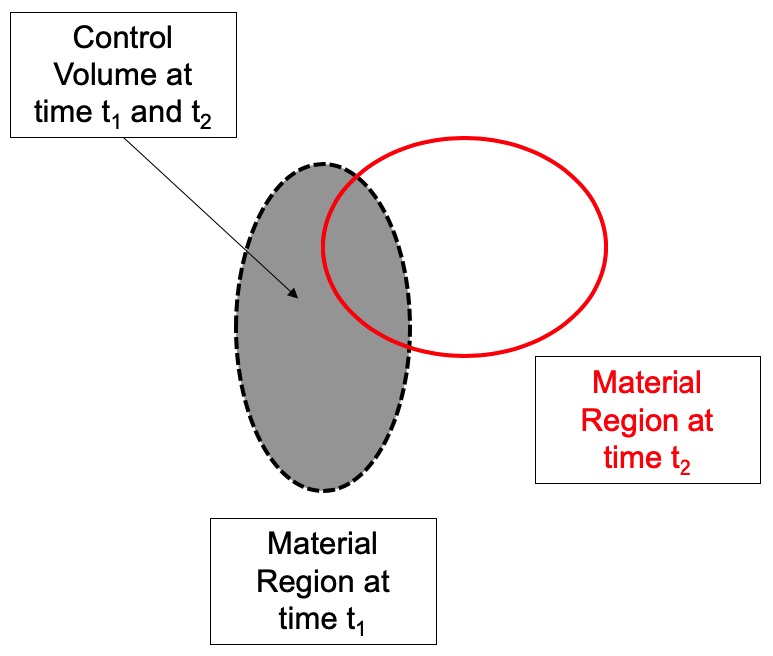
\includegraphics[height=2in]{Fund1.png}
   \caption{Material region and control volume. Black-dashed and red-circled region are the
   two material region at two time moments. The gray area overlaps with the material region at $t_1$
   and represents the control volume which is fixed regardless of time.}
   \label{figfund1}
\end{figure}

Let's express the mass conservation in the format of {\bf integral equation}:

\begin{align}\label{eqmassMR}
   \frac{\partial}{\partial t}\int_{\Omega_M(t)}\rho d\Omega = 0
\end{align}

Here $\Omega_M$ stands the volume of the material region which can be changing with time $t$. $\rho$
is the density and a function of time and space, and $d\Omega$ is a infinitesimal volume in 3D.
Next, we want to re-write Eqn. \ref{eqmassMR} in the context of {\bf control volume}, instead of
the material region. A control volume is a fixed volume of space and
do not change with time. Mass can flow into or out of the control volume. Typically, we only care a
specific type of control volume. That is the cells we introduced in chapter \ref{c1}. We will be
dealing with tons of control volumes as each cell represents a fixed volume of space and is viewed
as one control volume. The difference of control volume and material region should be emphasized.
The material region is the volume of space that encompasses a certain set of particles being
tracked, so the material region changes with time depending on the velocities of the particles. The
control volume is a fixed volume of space, and particles can freely flow into or out of the control
volume. Technically, the control volume can also be set to be moving, but let's just set it to be
stationary all the time. These two concepts represent two perspectives of describing the mechanics
of particles. The material region is called the {\bf Lagrangian point of view} and the control
volume is referred to as the {\bf Eulerian point of view}.
\paraspace

How to bridge the two point of views of describing mechanics? Let's find a time moment where the
material region and control volume are overlaid on one another, as shown in Fig. \ref{figfund1}.
If we take the Eulerian perspective, the mass within the {\bf control volume} should be changing
and the rate should be equal to the net mass rate flowing into/out of the control volume. Therefore,
writing in the format of integral equation, we have:

\begin{align}\label{eqmassCV}
   \int_{\Omega}\frac{\partial \rho}{\partial t}d\Omega + \int_{\partial \Omega}\rho (V\cdot n)
   d\sigma = 0
\end{align}

Here $\Omega$ is the control volume (we dropped the subscript $M$ to differentiate control volume
and material region). Note that we can move the partial derivative inside the integral since
$\Omega$ does not change with time. $\rho$ is still density as a function of time and space. $V$ is
the velocity (a 3D vector) and $n$ is the normal unit vector (also a 3D vector) on the 2D boundary
of the 3D control volume (written as $\partial \Omega$. The dot product $V\cdot n$ represents the
normal component of velocity on the boundary $\partial \Omega$. Finally, $d\sigma$ stands for the
infinitesimal surface area on $\partial \Omega$. One note regarding notation, we do not use the
arrow or bold font to differentiate vector, tensor and scalar. This clarity of the notation is
sacrificed to trade for conciseness in our equations.  \paraspace

The two equations Eqn. \ref{eqmassMR} and \ref{eqmassCV} are equivalent to each other. They
describe the same conservation law of mass but with two point of views. Eqn.
\ref{eqmassMR} is the Lagrangian view and Eqn. \ref{eqmassCV} is the Eulerian view. We will only use
the Eulerian point of view of describe fluid mechanics. The equivalence of the two point of views
can be proved mathematically based on the Leibnitz's theorem \cite{panton2013incompressible}. The
Leibnitz's theorem states that for any quantity $Q$:

\begin{align}\label{eqLeib}
   \frac{\partial}{\partial t}\int_{\Omega_M(t)}Q d\Omega = \int_\Omega \frac{\partial Q}{\partial
   t}d\Omega + \int_{\partial\Omega}Q (V\cdot n)d\sigma
\end{align}

In the context of fluid mechanics, $Q$ can be mass, momentum and energy.
\paraspace

\clearpage
\section{Governing equations}

For now on, we will be focusing on using control volume to describe the conservation equations
(Eulerian viewpoint). We have already introduced the mass conservation equation as Eqn.
\ref{eqmassCV}. Next, momentum conservation. In 3D, the momentum along the three dimensions should
all be ``conserved'' which gives 3 momentum conservation equations. Unlike the mass conservation,
the momentum of the control volume can be changed by forces. This is Newton's second law. We write
the integral form of momentum conservation equation as:


\begin{align}\label{eqmom}
   \int_\Omega \frac{\partial(\rho V_i)}{\partial t}d\Omega + \int_{\partial\Omega}(\rho
   V_i)(V\cdot n)d\sigma = \int_\Omega \rho f_i d\Omega + \int_{\partial\Omega}R_i d\sigma
\end{align}

On the left-hand-side (LHS), the first term is the temporal rate of the momentum along the $i$ dimension
($i = x, y, z$), integrated over the control volume.  The second term is the momentum flowing into
or out of the control volume. Note that the entire left-hand-side can be interpreted in the
Lagrangian viewpoint as the temporal rate of momentum of the {\bf material region}. Use Leibnitz's
theorem, Eqn. \ref{eqLeib}. The right-hand-side stands for the force. The first term on the
right-hand-side (RHS) is the {\bf body force} (the component along the $i$ direction), while the second
term is the {\bf surface force}. We note that the body force has the unit of $\textrm{N/kg}$ or the
unit of acceleration $\mathrm{m^2/s}$. The surface force has the unit of $\mathrm{N/m^2}$. The most
common body force is the gravitational force $g = [0, -9.81, 0]^T$
\paraspace

The surface force needs our special attention. To describe a surface force, we need to use {\bf
stress tensor}. Surface force can be alternatively referred to as the surface stress. Stress tensor
is a matrix $T$, and the surface force is given by $R = Tn$. This is a matrix multiplication where
$n$ and $R$ are column vectors. We will assume throughout this document a vector is a column vector,
unless otherwise specified. This can also be written as $R = (n\cdot T)^T$. I will avoid using
matrix multiplications and instead use dot products (inner product) or outer product in this
document. Note the dot (inner) product of matrices $A$ and $B$ are defined as $A \cdot B = A^T B$.
The multiplication of two matrices can be expressed as $AB = A^T \cdot B$. The outer product of two
matrices are defined as: $A\mathop{\otimes}B = AB^T$. \paraspace

The stress tensor has two components, pressure and viscous stress, expressed as:

\begin{align*}
   T = -p I + \tau
\end{align*}

where $p$ is the {\bf thermodynamic pressure}, $I$ is a 3 by 3 unit matrix (in 3D), and $\tau$ is the
viscous stress tensor which is a matrix as a function of the gradient of velocities. This
relationship is referred to as {\bf constitutive relations} which will be discussed later.
\paraspace

Next, let's consider the conservation of energy. Again, writing as integral equation:

\begin{align}\label{eqeng}
   \int_\Omega\frac{\partial(\rho e_{tot})}{\partial t} d\Omega + \int_{\partial\Omega}(\rho
   e_{tot}) (V \cdot n) d\sigma = \int_\Omega \rho f \cdot V d\Omega + \int_{\partial\Omega} (n\cdot
   T)^T \cdot V d\sigma - \int_{\partial\Omega}(n \cdot q) d\sigma
\end{align}

Here $e_{tot}$ is the {\bf total energy}, $e_{tot} = e + \tfrac{1}{2}V^2$, where $e$ is the
{\bf specific} internal energy, or energy per unit mass. The two terms combined on the LHS stands
for the temporal rate of total energy of the mass region, again, Leibnitz's theorem (Eqn
.\ref{eqLeib}). The first two terms on the RHS stand for the {\bf work} done by the body force and
surface force per unit time, or the {\bf power}. The last term of the RHS stands for the heat
transfer, or heat flux flowing into or out of the control volume, where $q$ is the heat flux vector
(with the unit of $W/m^2$. The heat flux is a function of temperature gradient. Such a relationship
is also part of the constitutive relations. The long equation (Eqn. \ref{eqeng}) is nothing other
than the {\bf first law of thermodynamics}, written as ``$dU = \delta Q - \delta W$'' in typical
thermodynamic textbooks.
\paraspace

Eqn. \ref{eqmassCV}, \ref{eqmom}, and \ref{eqeng} constitutes the {\bf governing equations} of
fluid mechanics, written in the form of integral equations. This set of equations is the basic set
while more governing equations need to be included when considering additional physics, e.g.,
conservation of chemical species. That being said, we limit our discussion to this set of basic
equations in this chapter.
\paraspace

\clearpage
\section{Constitutive Relations}

There are essentially five equations from Eqn. \ref{eqmassCV}, \ref{eqmom}, and \ref{eqeng}.
Therefore, we need to pick five independent variables, referred to as the {\bf primitive variables},
and express all the variables in Eqn.  \ref{eqmassCV}, \ref{eqmom}, and \ref{eqeng} as functions
of the independent. Such relations are generally referred to as the {\bf constitutive relations}. We
will be exclusively using $(p, V, T)$ as the primitive variables in this document. Note that the
choice of primitive variables can be arbitrary, but different choice may lead to entirely different
constitutive relations. The choice of $(p, V, T)$ is because that it is a convention to express
other properties of a material as functions of $p, V, T$ in, for example, material handbooks and
databases.
\paraspace

The {\bf thermodynamic relations} include $e = e(p, T)$ (internal energy), $\rho = \rho(p, T)$, and
sometimes the {\bf enthalpy}, $h = e + p/\rho$. The {\bf total enthalpy} can be expressed as
$h_{tot} = h + \tfrac{1}{2}V^2$. These relations are for the ``state functions'' and are often
referred to as the {\bf equation of state} (EOS).
\paraspace

The {\bf kinetic relations} describe the ``transfer'' of some quantity. For example, the transfer of
heat is described by the {\bf Fourier's law}:

\begin{align*}
   q = -k\nabla T
\end{align*}

where $k$ is the thermal conductivity. Note that $k$ is referred to as (one of) the {\bf transport
properties} and can be a function of primitive variables, $k = k(p,T)$. Also, Fourier's law only
governs the {\bf conduction} of heat transfer. Convection and radiation can be introduced by
including additional kinetic relations. But this is beyond the scope of the current discussion. The
transfer of momentum is described by the {\bf Newton's viscosity law}:

\begin{align*}
   \tau = \left(-\frac{2}{3}\mu \nabla \cdot V\right) I + 2 \mu S
\end{align*}

where $\mu$ is the viscosity and can be a function of primitive variables, $\mu = \mu(p, T)$.
$\nabla \cdot V$ is the divergence of velocity. Note that the nabla operator can be also treated as
a column vector: $\nabla = [\partial/\partial x, \partial/\partial y, \partial/\partial z]^T$.
Again, $I$ is a 3 by 3 unit matrix, and $S$ is the {\bf strain rate tensor}:

\begin{align}\label{eqstrainrate}
   S = 
   \begin{bmatrix}
      \frac{\partial u}{\partial x} & \frac{1}{2}(\frac{\partial v}{\partial x}+\frac{\partial
      u}{\partial y}) & \frac{1}{2}(\frac{\partial w}{\partial x} + \frac{\partial u}{\partial z})
      \\ \frac{1}{2}(\frac{\partial u}{\partial y} + \frac{\partial v}{\partial x}) & \frac{\partial
      v}{\partial y} & \frac{1}{2}(\frac{\partial w}{\partial y} + \frac{\partial v}{\partial z}) \\
      \frac{1}{2}(\frac{\partial u}{\partial z} + \frac{\partial x}{\partial w}) &
      \frac{1}{2}(\frac{\partial w}{\partial y} + \frac{\partial v}{\partial z}) &  \frac{\partial
      w}{\partial z} \\
   \end{bmatrix}
\end{align}

where $(u,v,w)$ are the three components of the velocity vector $V$. We can then express the
viscous stress as:

\begin{align}\label{eqviscousstress}
   \tau = \mu 
   \begin{bmatrix} 
      \frac{4}{3}\frac{\partial u}{\partial x} - \frac{2}{3}(\frac{\partial v}{\partial y} +
      \frac{\partial w}{\partial z}) & \frac{\partial v}{\partial x}+\frac{\partial u}{\partial y} &
      \frac{\partial w}{\partial x} + \frac{\partial u}{\partial z} \\ \frac{\partial u}{\partial y}
      + \frac{\partial v}{\partial x} & \frac{4}{3}\frac{\partial v}{\partial
         y}-\frac{2}{3}(\frac{\partial u}{\partial x} + \frac{\partial w}{\partial z}) &
         \frac{\partial w}{\partial y} + \frac{\partial v}{\partial z} \\ \frac{\partial u}{\partial
         z} + \frac{\partial x}{\partial w} & \frac{\partial w}{\partial y} + \frac{\partial
         v}{\partial z} & \frac{4}{3}\frac{\partial w}{\partial z} - \frac{2}{3}(\frac{\partial
      u}{\partial x} +\frac{\partial v}{\partial y})\\
   \end{bmatrix}
\end{align}



One final note regarding the
thermodynamic and kinetic relations. The term ``thermodynamic'' and ``kinetic'' are from material
science. Basically, ``thermodynamic'' is associated with the states of equilibrium while
``kinetic'' is associated with the states in between equilibrium, and therefore, with the gradient
of thermodynamic properties. This is a hand-wavy distinction of these two categories of constitutive
relations, based on concepts in material science.
\paraspace

Up to now, we can express all the quantities in Eqn. \ref{eqmassCV}, \ref{eqmom}, and \ref{eqeng}
as functions of the primitive variables $(p,V,T)$. The body force $f$ may be the exception, but for
now we can simply view it as a constant as for the gravitational force.
\paraspace

\clearpage
\section{Differential Governing Equations}

In this section we brief discuss the differential form of governing equations. Although this form is
not our focus in numerical implementations, it can be convenient to use this form in analysis. To
derive the differential form, we need to use Gauss's theorem

\begin{subequations}\label{eqGaussthm}
   \begin{align}
      &\int_\Omega \nabla \phi \; d\Omega = \int_{\partial\Omega} n\phi \; d\sigma, \quad \phi \textrm{
         is scalar} \\
      &\int_\Omega \nabla \cdot v \; d\Omega = \int_{\partial\Omega} n \cdot v \; d\sigma, \quad v \textrm{
         is vector} \\
      &\int_\Omega \nabla \cdot T \; d\Omega = \int_{\partial\Omega} n \cdot T \; d\sigma, \quad T \textrm{
         is matrix (tensor)}
   \end{align}
\end{subequations}

Again, the nabla operator is treated as a column vector $\nabla = [\partial/\partial x,
\partial/\partial y, \partial/\partial z]^T$, and note the LHS and RHS of Eqn. \ref{eqGaussthm}c
are both row vectors. Eqn. \ref{eqGaussthm}c can be transposed to give the column vector form.
\paraspace

Now, we can use Eqn. \ref{eqGaussthm} to transform the surface integrals to volume integrals in
Eqn. \ref{eqmassCV}, \ref{eqmom}, and \ref{eqeng}. Then, we can drop the integral and keep the
intergrand to obtain the differential equations. For example, the mass conservation can be written
as:

\begin{align}\label{eqmassDf}
   \frac{\partial \rho}{\partial t} + \nabla \cdot (\rho V) = 0
\end{align}

by applying Eqn. \ref{eqGaussthm}b and let $v = \rho V$. To derive momentum conservation equation,
we need to group the terms inside the surface integral to form tensors. First, we write Eqn.
\ref{eqmom} as:

\begin{align}\label{eqmomTs}
   \int_\Omega \frac{\partial(\rho V)}{\partial t}d\Omega + \int_{\partial\Omega} \left(n \cdot (\rho
   V \mathop{\otimes} V)\right)^T d\sigma = \int_\Omega \rho f d\Omega + \int_{\partial\Omega} (n
   \cdot T)^T d\sigma
\end{align}

where $T = -pI + \tau$, and note that $\rho V \mathop{\otimes} V$ is a matrix. Then, apply Eqn.
\ref{eqGaussthm}c to the surface integrals to get:

\begin{align}\label{eqmomDf}
   \frac{\partial (\rho V)}{\partial t} + \left(\nabla \cdot (\rho V \mathop{\otimes} V)\right)^T = \rho f
   + (-\nabla p) + (\nabla \cdot \tau)^T
\end{align}

Note that we applied the transpose operation to keep very vector as a column vector. Finally, to
derive the energy conservation equation, we observe that the work done by the surface force can be
rewritten as $(n \cdot T)^T \cdot V = n \cdot (T^T \cdot V)$. That is, the dot product of $n$ and
some matrix. Therefore, we can apply Eqn. \ref{eqGaussthm}c and obtain:

\begin{align}\label{eqengDf}
   \frac{\partial (\rho e_{tot})}{\partial t} + \nabla \cdot (\rho e_{tot} V) = \rho f \cdot V +
   (-\nabla \cdot (pV)) + \nabla \cdot (\tau^T \cdot V) - \nabla \cdot q
\end{align}

Now we have the set of differential equations, Eqn. \ref{eqmassDf}, \ref{eqmomDf}, and
\ref{eqengDf}, that governs the conservation of mass, momentum and
energy.
\paraspace

\clearpage
\section{Matrix Representation}

In this section, we will prepare the set of governing equations in integral form, Eqn.
\ref{eqmassCV}, \ref{eqmomTs}, and \ref{eqeng} in a format that is more suitable for numerical
computation. Let's first seperate the pressure and the viscous stress from the surface stress tensor
$T$, and rewrite the equations as follows:

\begin{subequations}\label{eqmatgov1}
   \begin{align}
      \int_{\Omega}\frac{\partial \rho}{\partial t}d\Omega + \int_{\partial \Omega} n \cdot (\rho V)
      d\sigma &= 0 \\
      \int_\Omega \frac{\partial(\rho V)}{\partial t}d\Omega + \int_{\partial\Omega} \left(n \cdot
      (\rho V \mathop{\otimes} V)\right)^T d\sigma & = \int_{\partial\Omega} (n \cdot (-p I))^T d\sigma +
      \int_{\partial\Omega} (n \cdot \tau)^T + \int_\Omega \rho f d\Omega \\
      \begin{split}
         \int_\Omega\frac{\partial(\rho e_{tot})}{\partial t} d\Omega + \int_{\partial\Omega} n \cdot
         (\rho e_{tot} V) d\sigma & = \int_{\partial\Omega} n\cdot (-p V) d\sigma + \int_{\partial\Omega}
         n \cdot (\tau^T \cdot V) d\sigma - \int_{\partial\Omega}(n \cdot q) d\sigma \\
         & + \int_\Omega \rho f
         \cdot V d\Omega 
      \end{split}
   \end{align}
\end{subequations}

Notice that for the energy equation Eqn. \ref{eqeng}, we used:

\begin{align*}
   (n \cdot T)^T \cdot V = n \cdot (T^T \cdot V) = n \cdot ((-p I + \tau^T) \cdot V) = n \cdot (-pV) + n
   \cdot (\tau^T \cdot V)
\end{align*}

We observe a similarity in Eqns \ref{eqmatgov1} that all the surface integrals has the form of the
norm vector $n$, dot product with some vector or tensor. Also, we want to distinguish the terms
related to gradients (e.g., $\tau$ and $q$) from those which does not. For that, we can move the
pressure-related terms from the RHS to the LHS to give:

\begin{subequations}\label{eqmatgov2}
   \begin{align}
      \int_{\Omega}\frac{\partial \rho}{\partial t}d\Omega + \int_{\partial \Omega} n \cdot (\rho V)
      d\sigma &= 0 \\ \int_\Omega \frac{\partial(\rho V)}{\partial t}d\Omega + \int_{\partial\Omega}
      \left(n \cdot (\rho V \mathop{\otimes} V + pI)\right)^T d\sigma & = \int_{\partial\Omega} (n
      \cdot \tau)^T + \int_\Omega \rho f d\Omega \\ \int_\Omega\frac{\partial(\rho e_{tot})}{\partial
      t} d\Omega + \int_{\partial\Omega} n \cdot (\rho h_{tot} V) d\sigma & = \int_{\partial\Omega} n
      \cdot (\tau^T \cdot V) d\sigma - \int_{\partial\Omega}(n \cdot q) d\sigma  + \int_\Omega \rho f
      \cdot V d\Omega 
   \end{align}
\end{subequations}

Note that for Eqn. \ref{eqmatgov2}c, we used $\rho e_{tot} + p = \rho h_{tot}$. Now, with the form
of Eqn. \ref{eqmatgov2}, we can group terms together to give the {\bf matrix representation} of the
governing equations:

\begin{align}\label{eqmatgov3}
   \int_{\Omega}\frac{\partial Q_c}{\partial t}d\Omega +  \int_{\partial \Omega} (n \cdot F_c)^T
   d\sigma = \int_{\partial \Omega} (n \cdot F_v)^T d\sigma + \int_{\Omega} S d\Omega
\end{align}

where the terms in Eqn. \ref{eqmatgov3} are as follows:

\begin{align*}
   &Q_c = \begin{bmatrix} 
      \rho \\
      \rho V \\
      \rho e_{tot}
   \end{bmatrix}_{5\times1} \quad 
   F_c = \begin{bmatrix} \rho V & \rho V\mathop{\otimes}V + pI & \rho h_{tot} V
      \end{bmatrix}_{3\times5} \\
      &F_v = \begin{bmatrix}0 & \tau & \tau^T \cdot V -
   q\end{bmatrix}_{3\times5} \quad S = \begin{bmatrix}
      0 \\
      \rho f \\
      \rho f \cdot V
      \end{bmatrix}_{5\times1}
\end{align*}

Again, all the vectors are expressed as column vectors. Eqn. \ref{eqmatgov3} can also be succinctly
written as:

\begin{align}\label{eqmatgov}
   \int_{\Omega}\frac{\partial Q_c}{\partial t}d\Omega +  \int_{\partial \Omega} (n \cdot (F_c -
   F_v))^T d\sigma = \int_{\Omega} S d\Omega
\end{align}

The corresponding differential form of the matrix representation can be derived by simply applying
Eqn. \ref{eqGaussthm}c:

\begin{align}\label{eqmatgovDf}
   \frac{\partial Q_c}{\partial t} + (\nabla \cdot (F_c - F_v))^T = S
\end{align}

Eqn. \ref{eqmatgovDf} is the one used in \cite{li2006unified}, but the integral form will be the
foundation for numerical computation. \paraspace 

Now let's briefly discuss the importance of such matrix representation Eqn. \ref{eqmatgov}. Here,
$Q_c$ is referred to as the {\bf conservative variables}, $F_c$ the {\bf convective flux}, $F_v$ the
{\bf viscous flux} and $S$ the source term. It is a succinct representation of a general form of
conservation law. It states that the temporal rate of a vector variable $Qc$  is due to the fluxes
due to translation of such variable ($F_c$), the gradient of such variable ($F_v$) as well as the
external source addition/destruction of such variable ($S$). With this form, we can conveniently add
more conservative variables to the vector $Q_c$ and modify accordingly the convective flux, viscous
flux and the source term. \paraspace

The control volume $\Omega$ in Eqn. \ref{eqmatgov} will be millions of cells in the mesh. For each
cell, we write down Eqn. \ref{eqmatgov}, with 5 unknowns in $Q_c$. Then, we will have millions of
unknowns and millions of equations for the entire calculation domain. Notice that the boundary of
the cell $\partial \Omega$ will be composed of faces. This foreshadows the surface integrals on the
boundary of a cell will be approximated by summations over the faces of the cell. \paraspace

It is more convenient to deal with the primitive variables $Q_p = [p, V, T]^T$, rather than the
conservative variables $Q_c$. Therefore, we can express Eqn. \ref{eqmatgov} as:

\begin{align}\label{eqgovready}
   &\int_{\Omega}\Gamma \frac{\partial Q_p}{\partial t}d\Omega + \int_{\partial \Omega} (n \cdot
   (F_c(Q_p) - F_v(Q_p)))^T d\sigma = \int_{\Omega} S(Q_p) d\Omega, \; \textrm{where }\Gamma = \frac{\partial Q_c}{\partial Q_p}
\end{align}

That is, expressing every term as functions of the primitive variable $Q_p$. Here, $\Gamma$ is referred
to as the {\bf conservative jacobian} which connects primitive variable and conservative variable.
\paraspace

\clearpage
\section{Preconditioning: Motivation}

In this section, we introduce some analysis on the system of governing equations Eqn.
\ref{eqmatgov} or \ref{eqmatgovDf} and reveal its properties. Importantly, the governing equations
can be viewed as a superimposition of wave equations, each with its propagation speed. We shall see
that the propagation speed of different waves can have drastically different magnitude under certain
circumstances (subsonic flow). In this scenario, the different wave speeds give difficulties in
numerically solving the governing equations. This problem is referred to as the {\bf
ill-conditioning} of the system, and we will introduce the {\bf preconditioning} method to such
difficulties.  \paraspace

First, let's reveal the wave-nature of the governing equations by considering the differential form
of the {\bf one-dimensional Euler equation} which is often used for analysis. Starting from Eqn.
\ref{eqmatgovDf}, we make the equations 1D, and remove the viscous flux (inviscid flow) and the
source term (neglected gravity), and obtain the following equation:

\begin{align}\label{eq1DEuler}
   \frac{\partial Q_c}{\partial t} + \frac{\partial E}{\partial x} = 0; \quad Q_c =
   \begin{bmatrix}\rho \\ \rho u \\ \rho h_{tot} - p\end{bmatrix}; \quad E =
      \begin{bmatrix}\rho u \\ \rho u^2 + p \\ \rho h_{tot} u\end{bmatrix}
\end{align}

Here, $E$ is the 1D convective flux and $u$ is the 1D velocity. Notice that we used $\rho h_{tot} -
p = \rho e_{tot}$ to replace any internal energy related terms with enthalpy related terms. This is
simply a convention that enthalpy is more popular than internal energy in material properties
handbooks. It should be pointed out that although the 1D Euler equation Eqn. \ref{eq1DEuler} is
significantly simplified from the original differential governing equation Eqn. \ref{eqmatgovDf},
the essence of the governing equation is retained. It will be straightforward to show that the 1D
Euler equation is a superimposition of wave equations.\paraspace

Now let's use primitive variable $Q_p = [p, u, T]^T$ to express the 1D Euler equation as:

\begin{align}\label{eq1DEulerP1}
   \Gamma \frac{\partial Q_p}{\partial t} + A_c \frac{\partial Q_p}{\partial x} = 0; \quad \Gamma =
   \frac{\partial Q_c}{\partial Q_p}, \; A_c = \frac{\partial E}{\partial Q_p}
\end{align}

where $A_c$ is the {\bf convective flux jacobian} and $\Gamma$ is the conservative jacobian. These
jacobians can be explicitly evaluated by taking the partial derivatives of material properties with
respect to the primitive variables, as follows:

\begin{align*}
   &\Gamma = \begin{bmatrix}
      \rho_p & 0 & \rho_T \\
      \rho_p u & \rho & \rho_T u \\
      \rho_p h_{tot} + \rho h_p - 1 & \rho u & \rho_T h_{tot} + \rho h_T
   \end{bmatrix} \\
   &A_c = \begin{bmatrix}
      \rho_p u & \rho & \rho_T u \\
      \rho_p u^2 + 1 & 2\rho u & \rho_T u^2 \\
      (\rho_p h_{tot} + \rho h_p)u & \rho h_{tot} + \rho u^2 & (\rho_T h_{tot} + \rho h_T)u
      \end{bmatrix}
\end{align*}

Here we used subscript notation $a_b$ to represent the partial derivative of $b$ with respect to
$a$. We point out that there are in total 4 partial derivatives in $\Gamma$ and $A_c$ which are
$\rho_p$, $\rho_T$, $h_p$ and $h_T$. They all have significant physical meanings and are fairly
accessible in material property handbooks.\paraspace

We can further simply Eqn. \ref{eq1DEulerP1} by multiplying the LHS with $\Gamma^{-1}$ and group
$\Gamma^{-1}A_c$ to be a matrix $A$:

\begin{align}\label{eq1DEulerP2}
   \frac{\partial Q_p}{\partial t} + A \frac{\partial Q_p}{\partial x} = 0; \quad A = \Gamma^{-1}A_c
\end{align}

Eqn. \ref{eq1DEulerP2} already has the ``form'' of a wave equation. Notice that the three
components of $Q_p$ are intertwined through the matrix $A$, typically referred to as the {\bf
system matrix} of a wave equation. This coupling can be removed by performing the diagonalization of
the system matrix $A$:

\begin{align*}
   A = M \Lambda M^{-1}; \quad \Lambda = \textrm{diag}\{\lambda_1, \lambda_2, \lambda_3\}
\end{align*}

Here $\Lambda$ is a diagonal matrix storing the eigenvalues of $A$ and $M$ stores the eigenvectors
in its column vectors. Note that both $\Lambda$ and $M$ are analytical expression that can be
explicitly evaluated. Next, we manufacture a variable $\widehat{Q}$, such that:

\begin{align*}
   M = \frac{\partial Q_p}{\partial \widehat{Q}}
\end{align*}

This is to transform Eqn. \ref{eq1DEulerP2} to:

\begin{align*}
   M\frac{\partial \widehat{Q}}{\partial t} + AM\frac{\partial \widehat{Q}}{\partial x} = 0
\end{align*}

Then, multiply the LHS by $M^{-1}$ and realize $\Lambda = M^{-1}AM$ to obtain:

\begin{align}\label{eq1DEulerCh}
   \frac{\partial \widehat{Q}}{\partial t} + \Lambda\frac{\partial \widehat{Q}}{\partial x} = 0
\end{align}

We refer $\widehat{Q}$ as the {\bf characteristic variable}. Note that $\widehat{Q}$ is purely
manufactured and does not necessarily have any physical meaning. It is defined by a differential
relation with $Q_p$ and in most of the cases, does not even have a closed-form expression. However,
by transforming $Q_p$ to $\widehat{Q}$, the wave nature of the governing equation can be better
revealed as in Eqn. \ref{eq1DEulerCh}. We can also write it as: 

\begin{align*}
   \begin{cases}
      \frac{\partial \widehat{q}_1}{\partial t} + \lambda_1 \frac{\partial \widehat{q}_1}{\partial
      x} = 0 \\ 
      \frac{\partial \widehat{q}_2}{\partial t} + \lambda_2 \frac{\partial
      \widehat{q}_2}{\partial x} = 0 \\
      \frac{\partial \widehat{q}_3}{\partial t} + \lambda_3 \frac{\partial
      \widehat{q}_3}{\partial x} = 0 \\
   \end{cases}
\end{align*}

As we can see, each component of the characteristic variable, $\widehat{q}_i$ ($i=1,2,3$) propagates
like a wave with the propagation speed of $\lambda_i$. If $\lambda_i$ were constant (or
approximately as constant), these would have been 1D linear wave equations with analytical solution.
In such a case, Eqn. \ref{eq1DEulerP2} can be solved (or approximately solved) by transforming back
from $\widehat{Q}$ to $Q_p$.\paraspace

In reality, $\lambda_i$'s are not constant. They can be expressed as some functions of the primitive
variable. These functions can be derived by diagonalizing the system matrix $\Gamma^{-1}A_c$.
Unfortunately, such a derivation will be extremely tedious as the system matrix is composed of long
expressions of the primitive variable. Therefore, this task is usually done by symbolic
operations of some computer program such as MATLAB. After doing so, the wave propagation speeds
$\lambda_i$'s are found out to be:

\begin{subequations}\label{eqwavespeed}
   \begin{align}
      &\lambda_1 = u \\
      &\lambda_2 = u + \sqrt{\frac{\rho h_T}{\rho_T + \rho h_T \rho_p - \rho h_p \rho_T}} \\
      &\lambda_3 = u - \sqrt{\frac{\rho h_T}{\rho_T + \rho h_T \rho_p - \rho h_p \rho_T}}
   \end{align}
\end{subequations}

The {\bf acoustic speed}, or {\bf sound speed} can be defined as:

\begin{align}\label{eqsoundspeed}
   c = \sqrt{\frac{\rho h_T}{\rho_T + \rho h_T \rho_p - \rho h_p \rho_T}}
\end{align}

such that the three wave speeds are:

\begin{align*}
   \lambda_1 = u, \; \lambda_2 = u+c, \; \lambda_3 = u-c
\end{align*}

We refer to the wave associated with $\lambda_1$ as the {\bf particle wave} because its propagation
speed is equal to the transnational velocity of particles of the material, $u$. We refer to the
waves associated with $\lambda_2$ and $\lambda_3$ as the {\bf acoustic waves} as they involves the
intrinsic acoustic property of the material, the sound speed $c$. \paraspace

It follows from Eqn. \ref{eqwavespeed} that, when the particle speed $u$ is comparable to the
acoustic speed $c$, all the wave speeds are comparable. This is the case in transonic and supersonic
flows typically studied in aerodynamics. However, if the particle speed $u$ is small compared to
$c$, as typical in subsonic flows, there can be a large difference between the wave speeds. Since
wave speeds are the eigenvalues of the system matrix $\Gamma^{-1}A_c$, the term ``ill-conditioned''
is borrowed from linear algebra to describe this situation, where the magnitude of eigenvalues of
a matrix is drastically different. \paraspace

The ill-conditioning of the system brings a variety of difficulties when numerically solving the
governing equation Eqn. \ref{eq1DEulerP1}. As we have not discussed any aspects regarding
numerical computation, we only qualitatively describe the difficulties here. One of the difficulties
is that the numerical errors tend to be magnified in an ill-conditioned system, which often
causes the code to crash. To avoid the crash, more incremental steps must be taken in the solution
process such that the errors in each step is small and can be contained. But this can significantly
increases the computational cost, or in other words, ``the code runs too slow''. These difficulties
are intrinsic due to the system eigenvalues having disparate magnitude. \paraspace

The philosophy of preconditioning is to alter the eigenvalues of the system such that all the
eigenvalues have comparable magnitude. To do that we modify the temporal term in the original
governing equation Eqn. \ref{eq1DEulerP1} to write:

\begin{align*}
   \Gamma_p \frac{\partial Q_p}{\partial t} + A_c \frac{\partial Q_p}{\partial x} = 0
\end{align*}

Note that the original conservative jacobian $\Gamma$ is modified as $\Gamma_p$. By doing so, the
new system matrix $\Gamma_p^{-1}A_c$ will have a new set of eigenvalues $\{\lambda_1, \lambda_2,
\lambda_3\}$ different than those in Eqn. \ref{eqwavespeed}. The new eigenvalues will have
comparable magnitude and make the system properly conditioned. \paraspace

One may be wondering whether the preconditioning has changed the governing equation, and therefore,
gives unphysical solutions. Not for the {\bf steady state solution} which does not change with time.
Indeed, for a steady state problem, the governing equation in Eqn. \ref{eq1DEulerP1} could be
written as:

\begin{align}\label{eq1DEulerss}
   A_c \frac{\partial Q_p}{\partial x} = 0
\end{align}

since $\partial Q_p / \partial t = 0$ for steady state solution. Therefore, altering the
conservative jacobian in the temporal term will not have any effects on the steady state solution.
For a steady state problem, the time evolution does not have to be physical, as long as the temporal
rate eventually vanishes and Eqn. \ref{eq1DEulerss} is satisfied. In this sense, the time evolution
in steady state problems can be understood as a {\bf pseudo time} evolution. We often use $\tau$
instead of the $t$ to emphasize this fact:

\begin{align*}
   \Gamma_p \frac{\partial Q_p}{\partial \tau} + A_c \frac{\partial Q_p}{\partial x} = 0
\end{align*}

and this strategy of solving steady state problems is referred to as the {\bf time marching
method}.\paraspace

But what if the solution is unsteady as $Q_p$ can evolve with time? The same philosophy can be
elegantly applied. We can introduce a second set of time evolution which, in its steady state,
approaches to the original unsteady governing equation. Such scheme is referred to as the {\bf dual
time scheme}. For example, we can write the governing equation as:

\begin{align*}
   \Gamma_p \frac{\partial Q_p^{n+1}}{\partial \tau} + \Gamma \frac{Q_p^{n+1} - Q_p^n}{\Delta t} + A_c
   \frac{\partial Q_p^{n+1}}{\partial x} = 0
\end{align*}

where $Q_p^n$ is the solution at the $n^{th}$ time moment $t^n$, which is assumed to be known.
$Q_p^{n+1}$ is the unknown to be solved at the next time moment $t^{n+1}$, and $\Delta t = t^{n+1} -
t^n$ is the time step size. Note that $Q_p^{n+1}$ is a function of $x$ and $\tau$ but is independent
of the physical time $t$, $Q_p^{n+1} = Q_p^{n+1} (x,\tau)$. In its steady state solution (of pseudo
time $\tau$), the temporal term vanishes, $\partial Q_p^{n+1} / \partial \tau = 0$, and the
governing equation goes back to:

\begin{align*}
   \Gamma \frac{Q_p^{n+1} - Q_p^n}{\Delta t} + A_c \frac{\partial Q_p^{n+1}}{\partial x} = 0
\end{align*}

Once we find the solution $Q_p^{n+1}$, we can proceed to the next physical time step. In the next
physical time step, again, we need to solve a steady state problem in the pseudo time $\tau$ to
obtain a solution $Q_p^{n+2}$, etc. The detailed discussion regarding the dual time scheme will be
given the next chapter.\paraspace


\chapter{Algorithm}

\section{Spatial and Explicit Temporal Discretization}

In this chapter, we will be using the data structure introduced in chapter \ref{c1} to solve the
governing equations introduced in chapter \ref{c2}. Specifically, the physical domain is discretized
by the mesh, e.g., in Fig. \ref{figmesh3}. Each cell is a control volume in which we can write the
governing equation, e.g., Eqn. \ref{eqgovready} by applying the cell volume as $\Omega$ and the
cell boundary (surrounding faces) as $\partial\Omega$. By doing so, the number of governing
equations we can write down is equal to the number of cells in the mesh. Now, we need to {\bf
discretize} the governing equation in order to produce numerical solutions. Let's first rewrite the
governing equations as (based on Eqn. \ref{eqmatgov3}, \ref{eqmatgov}, and \ref{eqgovready}):

\begin{align}\label{eqgovalg}
\begin{split}
   &\int_{\Omega} \Gamma \frac{\partial Q_p}{\partial t} d\Omega + \int_{\partial\Omega}
   [F_{cn}(Q_p, n) - F_{vn}(Q_p, n)] d\sigma = \int_{\Omega} S(Q_p) d\Omega \\
   &\textrm{where  } F_{cn} = \begin{bmatrix}\rho V_n \\ \rho V_n V + pn \\ \rho V_n
      h_{tot}\end{bmatrix}, \quad F_{vn} = \begin{bmatrix}0 \\ \tau \cdot n \\ n \cdot (\tau^T \cdot
   V) - n \cdot q\end{bmatrix}, \quad V_n = V \cdot n
\end{split}
\end{align}

Here we created the terms $F_{cn}$ and $F_{vn}$ for the convective and viscous flux along the normal
direction $n$ of the control volume surface. Note that we have two volume integrals and one surface
integral. We can use the {\bf volume-average} of primitive variable of each cell to approximate the
volume integrals:

\begin{subequations}\label{eqdisc1}
   \begin{align}
      &\int_{\Omega_I} \Gamma \frac{\partial Q_p}{\partial t} d\Omega \approx \Gamma(Q_{p,I}) \frac{\partial
      Q_{p,I}}{\partial t} \Omega_I \\
      &\int_{\Omega_I} S(Q_p) d\Omega \approx S(Q_{p,I}) \Omega_I
   \end{align}
\end{subequations}

Here we use capital letter $I$ to index the cells. $\Omega_I$ is the volume of the cell and
$Q_{p,I}$ is the volume-average of the primitive variable for cell $I$. For the surface integrals,
we want to use the volume-average of cell primitive variable to provide an approximation:

\begin{subequations}\label{eqdisc2}
   \begin{align}
      &\int_{\partial\Omega_I} F_{cn}(Q_p, n) d\sigma \approx \sum_{i \in I_{sf}} \mathcal{F}(Q_{pL,i},
      Q_{pR,i}, n_{Ii}) \sigma_i \\
      &\int_{\partial\Omega_I} F_{vn}(Q_p, n) d\sigma \approx \sum_{i \in I_{sf}} F_{vn}(Q_{p,i},
      (\nabla \mathop{\otimes} Q_p)_i, n_{Ii}) \sigma_i
   \end{align}
\end{subequations}

We use lower case letter $i$ to index the faces. Here, $I_{sf}$ is the set of faces surrounding cell
$I$, $Q_{pL,i}$ is referred to as the {\bf left state} of face $i$, $Q_{pR,i}$ is the {\bf right
state} of face $i$, $Q_{p,i}$ is the {\bf face-average} of primitive variable on the face $i$,
$(\nabla \mathop{\otimes} Q_p)_i$ is the {\bf face gradient} of primitive variable on the face $i$,
$n_{Ii}$ is the normal vector of face $i$ pointing {\bf out of} cell $I$, and finally, $\sigma_i$ is
the area of face $i$. Notice that there is a significant difference in the calculation of convective
and viscous flux. For the convective flux, a {\bf numerical flux function}, $\mathcal{F}$, is
defined which is different from the analytical expressions of $F_{cn}$ as in Eqn. \ref{eqgovalg}.
The computation of $\mathcal{F}$ will rely on the determination of the left and right state. For the
viscous flux, the analytical expression $F_{vn}$ as in Eqn. \ref{eqgovalg} is kept, and the
face-based terms, $Q_{p,i}$ and $(\nabla \mathop{\otimes} Q_p)_i$ need to be determined before the
viscous flux can be computed. We note that the approximation in Eqn. \ref{eqdisc2} utilizes the
face-based terms with a subscript $i$ while the approximation in Eqn. \ref{eqdisc1} utilizes the
cell-based terms with a subscript $I$. We emphasize that the cell-based terms will be first
calculated, and then, the face-based terms can be {\bf interpolated} from the cell-based terms.
\paraspace

The numerical flux function deserves some extra comments. To compute a numerical (convective) flux,
we first need to construct the left and right state with respect to a face. Next, the state
variables are plugged into the flux function $\mathcal{F}$ to produce the approximation of the
surface integrals in Eqn.  \ref{eqdisc2}.  The state variables can be simply the volume-average of
the left and right cells with respect to face $i$, denoted by $Q_{pl,i}$ and $Q_{pr,i}$. Notice we
use the lower case letter $l$ and $r$ to differentiate the state variables and the cell-average
variables. The more sophisticated choice of state variables involves some extrapolation from cells
to faces, which we will introduce later. The concept of left and right state comes from {\bf the
Riemann problem} \cite{toro2013riemann} and we will not expand here.  One can simply understand the
concept by relating to the fact that, to compute the face flux, we need both the information from
left and right side of the face. One should keep in mind that no matter how sophisticated the
construction of the state variables is, given all the cell-average $Q_{p,I}$'s, the left and right
state at every face $i$, $(Q_{pL,i}, Q_{pR,i})$ can be obtained. A final comment about the numerical
flux function $\mathcal{F}$. The design of such function is to approximate the face flux such that
the numerical solutions of $Q_p$ approaches the real solutions.  There can be many choices of such
flux functions and the design of numerical flux functions is an important topic of CFD. \paraspace

Through the spatial discretization in Eqn. \ref{eqdisc1} and \ref{eqdisc2}, we have replaced the
integrals in the governing equation by a bunch of summations. However, there is still a temporal
differentiation in the governing equation, which is not yet fully discretized. To perform the
temporal discretization, we approximate the differentiation by finite differences:

\begin{align}\label{eqdisct1}
   \Gamma(Q_{p,I})\frac{\partial Q_{p,I}}{\partial t} \approx \Gamma(Q_{p,I}^n) \frac{Q_{p,I}^{n+1} -
   Q_{p,I}^n}{\Delta t}
\end{align}

Notice that we add the superscript $n$ and indicate the discretized solution for cell $I$ at the
$n^{th}$ time moment as $Q_{p,I}^n$. $\Delta t$ is referred to as the {\bf time step} of the
numerical solution. We assume the time step size is constant although technically it can be changing
between the $n^{th}$ and the $(n+1)^{th}$ time moment. We point out that, by applying the temporal
discretization (Eqn. \ref{eqdisct1}), the numerical solution will consists of a time sequence
$\{Q_{p,I}^0, Q_{p,I}^1, Q_{p,I}^2, \cdots\}$ for each cell $I$. The {\bf initial condition} for
each cell, $Q_{p,I}^0$ is given, and based on the initial condition, the temporal evolution of
primitive variables in every cell will be solved incrementally by the numerical scheme.  \paraspace

The time discretization given by Eqn. \ref{eqdisct1} is of only first order in terms of finite
difference approximation. A second order approximation can be written as:

\begin{align}\label{eqdisct2}
   \Gamma(Q_{p,I})\frac{\partial Q_{p,I}}{\partial t} \approx \Gamma(Q_{p,I}^n) \frac{2Q_{p,I}^{n+1} -
   3Q_{p,I}^n + Q_{p,I}^{n-1}}{2\Delta t}
\end{align}

For the second order approximation, $Q_p$ at time moment $n$ and $(n-1)$ is given to compute $Q_p$
at time moment $(n+1)$. Accordingly, we need two initial conditions, we typically assume $Q_{p,I}^1
= Q_{p,I}^1$ to proceed to solve $Q_{p,I}^2$, $Q_{p,I}^3$, etc. In a more general context, we can
apply the $m^{th}$ order finite difference to the temporal discretization as:

\begin{align*}
   \Gamma(Q_{p,I})\frac{\partial Q_{p,I}}{\partial t} \approx \Gamma(Q_{p,I}^n) \sum_{j=n-m+1}^{1}
   g_j Q_{p,I}^{n+j}
\end{align*}

The coefficients $g_j$'s are referred to as the {\bf Gear's coefficients} for temporal
discretization. \paraspace

So far we only applied the temporal discretization to Eqn. \ref{eqdisc1}a, now we want to add the
superscript to the other terms in Eqn. \ref{eqdisc1}b and Eqn. \ref{eqdisc2} to complete the
spatial and temporal discretization. In the {\bf explicit time discretization}, we simply evaluate the
terms in Eqn. \ref{eqdisc1}b and Eqn. \ref{eqdisc2} at the current time moment, i.e., time moment
$n$, resulting in the fully discretized equation as:

\begin{align}\label{eqexp1}
   \begin{split}
      \Gamma(Q_{p,I}^n) \frac{2Q_{p,I}^{n+1} - 3Q_{p,I}^n + Q_{p,I}^{n-1}}{2\Delta t} \Omega_I +
      &\sum_{i \in I_{sf}} \mathcal{F}(Q_{pL,i}^n, Q_{pR,i}^n, n_{Ii}) \sigma_i - \\ &\sum_{i \in
      I_{sf}} F_{vn}(Q_{p,i}^n, (\nabla \mathop{\otimes} Q_p)_i^n, n_{Ii}) \sigma_i = S(Q_{p,I}^n)
      \Omega_I
   \end{split}
\end{align}

In Eqn. \ref{eqexp1}, the {\bf known} variables will be the primitive variables in each cell $I$,
at time $n$ and $n-1$, i.e., $Q_{p,I}^n$ and $Q_{p,I}^{n-1}$. The face-related variables (with
subscript $i$) can be interpolated/extrapolated based on the cell primitive variables. The {\bf
unknown} variables we aim to solve is the cell primitive variables at the next time step $n+1$,
$Q_{p,I}^{n+1}$. We can maneuver Eqn. \ref{eqexp1} such that all the unknowns are put on the LHS and
all the terms known are put on the RHS:

\begin{align}\label{eqlh1}
   \begin{split}
      & \L(\vec{Q}_p^n) \Delta \vec{Q}_p^n = \R(\vec{Q}_p^n), \\ & \textrm{where} \; \L_{II} =
      \frac{\Gamma(Q_{p,I}^n)\Omega_I}{\Delta t}, \; \L_{IJ} = 0 \; (I \neq J), \; \Delta \Q_p^n =
      \Q_p^{n+1} - \Q_p^n, \; \textrm{and } \\
      & \R_I = -\left(-\frac{\Gamma(Q_{p,I}^n) (Q_{p,I}^n - Q_{p,I}^{n-1})\Omega_I}{2\Delta t} +
         \right.\\
      &\left.\sum_{i \in
            I_{sf}}\left[\mathcal{F}(Q_{pL,i}^n, Q_{pR,i}^n, n_{Ii}) - F_{vn}(Q_{p,i}^n, (\nabla
\mathop{\otimes} Q_p)_i^n, n_{Ii})\right]\sigma_i\right) + S(Q_{p,I}^n)\Omega_I
   \end{split}
\end{align}

Here, the arrow on the variable, e.g., $Q_p^n$ indicates a vector containing $Q_p^n$ for all the
cells, and therefore, the subscript $I$ is dropped. For example, if the number of cells is 20, the
vector $\Q_p^n$ is a column vector with have 20 components: $[Q_{p,1}^n, \cdots Q_{p,20}^n]^T$, and
each component itself is a vector. For example, the 10\th component is $[p_{10}, V_{10}, T_{10}]^T$,
which is the pressure, velocity and temperature for the 10\th cell. In this case, the unknown vector
in Eqn.  \ref{eqlh1}, $\vec{Q}_p^n$, would have a length of 100 (in three dimension). To solve this
vector, we are basically dealing with a linear system where a matrix $\L$, multiples the unknown
vector $\vec{Q}_p^n$, equals to another vector $\R$. Again, assume $\vec{Q}_p^n$ has a length of 100
as an example, the matrix $\L$ would be $100 \times 100$ and the RHS vector $\R$ would be $100
\times 1$. We refer to $\L$ as the {\bf left-hand-side matrix}, or {\bf left-hand-side operator},
and refer to $\R$ as the {\bf right-side-side residual}, or simply the {\bf residual}. As indicated
in Eqn. \ref{eqlh1}, the LHS matrix in this case is a block diagonal matrix, while the residual is
a complex function of $\vec{Q}_p^n$ and $\vec{Q}_p^{n-1}$. However, since the LHS matrix is block
diagonal, we can simply invert $\L$ to solve $\Delta \Q_p^n$:

\begin{align*}
   \Delta \Q_p^n = \L^{-1}(\Q_p^n) \R(\Q_p^n)
\end{align*}

We can see that the original governing equations Eqn. \ref{eqgovalg}, which are integral equations, have
become a system of linear equations, after the spatial and temporal discretization. \paraspace

To close this section, let's briefly revisit the data structure and discuss how information
regarding Eqn. \ref{eqlh1} is stored. We add the following attributes to the \verb+cell+ type:

\begin{lstlisting}{language=[90]Fortran}
   type cell
      ...
      type(vector) :: qv, dqv
      type(matrix) :: dm
      type(vector) :: res
      type(vector) :: qvn(:)
   end type cell
\end{lstlisting}

where the type \verb+vector+ is another derived data type:

\begin{lstlisting}{language=[90]Fortran}
   type vector
      real :: v(neq)
   end type vector
\end{lstlisting}

The \verb+vector+ has one attribute which is a 1D array of floating point numbers. The variable
\verb+neq+ is a global variable indicating the number of governing equations in Eqn.
\ref{eqgovalg}. E.g., \verb+neq = 5+ in 3D and \verb+neq = 4+ in 2D, etc. The type \verb+matrix+ is
also a derived data type:

\begin{lstlisting}{language=[90]Fortran}
   type matrix
      real :: e(neq, neq)
   end type matrix
\end{lstlisting}

The \verb+matrix+ type has one attribute which is a 2D array of floating numbers. In the added
attributes of \verb+cell+, we will use \verb+qv+ to store the updated primitive variable
$Q_{p,I}^{n+1}$, \verb+dqv+ to store the increment $\Delta Q_{p,I}^n = Q_{p,I}^{n+1} -
Q_{p,I}^{n}$, and \verb+qvn+ to store the primitive variables in the previous time steps,
$Q_{p,I}^{n}$ and $Q_{p,I}^{n-1}$. Notice that \verb+qvn+ is an array of \verb+vector+. Its length
will depend on the order of the temporal discretization. In the case of second order as in Eqn.
\ref{eqexp1}, we need two previous time moments and the length of \verb+qvn+ will be two. Finally,
the attribute \verb+dm+ stores the diagonal terms of the LHS matrix $\L_{II}$ and the attribute
\verb+res+ stores the residual for the cell, $\R_I$. \paraspace

\clearpage
\section{Gradient Computation}

From now on, our discussion will be built on the key equation \ref{eqlh1} which is that a LHS
matrix $\L$ multiplies the unknown vector $\Delta Q_p$ equals to the residual $\R$. This chapter
will be devoted to the computation of gradients for both cells and faces. The gradients will be used
in the residual when calculating the left and right states, as well as in the viscous flux.
Specially, we are aiming at computing the following matrix:

\begin{align*}
   \nabla \mathop{\otimes} Q_p = \begin{bmatrix} \partial_x \\ \partial_y \\ \partial_z \end{bmatrix}
   \begin{bmatrix}p & u & v & w & T\end{bmatrix} = 
   \begin{bmatrix}
      \partial_x p &\partial_x u &\partial_x v &\partial_x w &\partial_x T \\
      \partial_y p &\partial_y u &\partial_y v &\partial_y w &\partial_y T \\
      \partial_z p &\partial_z u &\partial_z v &\partial_z w &\partial_z T 
   \end{bmatrix}
\end{align*}

Note that we use the short-hand notation $\partial_x p$ for $\partial p/\partial x$, etc. Also, $(u,
v, w)$ are the $(x,y,z)$ components of the velocity vector $V$. The gradient matrix $\nabla \o Q_p$
in this case is a $3 \times 5$ matrix. We will be computing such a matrix for each cell and face
given the primitive variable at each cell $Q_{p,I}$.

\subsubsection{Cell Gradient, Method 1: Least Mean Square}

Let's consider the pentagon cell $I$ shown in Fig. \ref{figcellg}. To include more generality, we
assume cell $I$ has 5 triangle neighboring cells, indexed as $I1, \cdots, I5$. The centroid of
the cells are labeled with $C$. We also draw 5 vectors from the centroid of cell $I$ to its
neighboring cells' centroid as $d_{I1}, \cdots, d_{I5}$. The objective is to compute the gradient
matrix at cell $I$, given that the primitive variables $Q_p$ are known at cell $I, I1, \cdots,
I5$.

\begin{figure}[H]
   \centering
   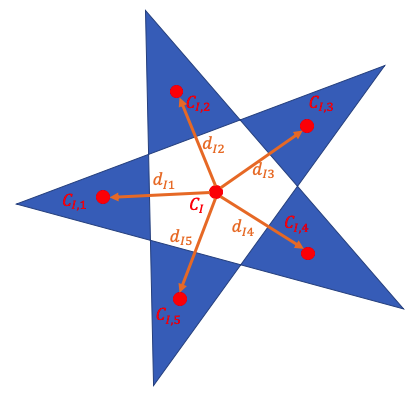
\includegraphics[height=3in]{Algorithm1.png}
   \caption{Illustration of cell gradient computation.}
   \label{figcellg}
\end{figure}

Let's take the gradient of pressure for example. Knowing $p_I, p_{I1}, \cdots, p_{I5}$, we can write
down the following approximation:

\begin{align}\label{eqlms1}
   \begin{split}
      &\begin{bmatrix}
         \Delta x_{I1} & \Delta y_{I1} & \Delta z_{I1} \\
         \Delta x_{I2} & \Delta y_{I2} & \Delta z_{I2} \\
         \Delta x_{I3} & \Delta y_{I3} & \Delta z_{I3} \\
         \Delta x_{I4} & \Delta y_{I4} & \Delta z_{I4} \\
         \Delta x_{I5} & \Delta y_{I5} & \Delta z_{I5}
      \end{bmatrix} \begin{bmatrix}\partial_x p \\ \partial_y p \\ \partial_z p\end{bmatrix} \approx
      \begin{bmatrix}\Delta p_{I1} \\\Delta p_{I2} \\\Delta p_{I3} \\\Delta p_{I4} \\\Delta p_{I5}
         \end{bmatrix} \\ &\textrm{where} \quad \begin{bmatrix}\Delta x_{IJ} & \Delta y_{IJ} &
      \Delta z_{IJ}\end{bmatrix} = d_{IJ}^T, J = 1,2,\cdots,5, \; \textrm{ and} \\ &\Delta p_{IJ} =
      p_{IJ} - p_I, J = 1,2,\cdots,5
   \end{split}
\end{align}

We can understand the task of computing the gradient of $p$ as the follows: find the gradient of $p$
such that the difference (error) between the LHS and RHS of Eqn. \ref{eqlms1} is minimized. This is
a {\bf Least Mean Square} (LMS) problem. That is, find the best vector $x$ that minimizes the
approximation $Ax \approx b$. In the case of Eqn. \ref{eqlms1}, $x$ is a $3\times1$ vector, $A$ is a
$5\times3$ matrix and $b$ is a $5\times1$ vector. The solution to the LMS problem is to find the
{\bf pseudo inverse} of matrix $A$, $A^+$, such that $x = A^+b$ produces the optimal $x$ minimizing
the approximation error. In the case of Eqn. \ref{eqlms1}, we can express the solution as:

\begin{align}\label{eqlms2}
   \begin{bmatrix}\partial_x p \\ \partial_y p \\ \partial_z p\end{bmatrix} = 
   \begin{bmatrix}
      s_{x1} &s_{x2} &s_{x3} &s_{x4} &s_{x5} \\ 
      s_{y1} &s_{y2} &s_{y3} &s_{y4} &s_{y5} \\ 
      s_{z1} &s_{z2} &s_{z3} &s_{z4} &s_{z5}
   \end{bmatrix}
   \begin{bmatrix}\Delta p_{I1} \\\Delta p_{I2} \\\Delta p_{I3} \\\Delta p_{I4} \\\Delta p_{I5}\end{bmatrix}
\end{align}

where the matrix with components $s$'s is the pseudo inverse of the matrix on the LHS on Eqn.
\ref{eqlms1}. For reasons to be illustrated, we shall refer to this matrix as the {\bf SVD} matrix.
The subscripts of $s$'s can be understood as some contributing weights. For example, $s_{y3}$ is the
contributing weights of the {\bf third} neighboring cell to the {\bf y} direction of the gradients,
etc. We note that the SVD matrix is only determined by the directional vectors $d_{IJ}$ in Fig.
\ref{figcellg} and Eqn. \ref{eqlms2} can be applied to any primitive variables besides $p$.
\paraspace

Now we shall present a general expression for computing the gradients of all primitive variables,
given that the pseudo inverse, i.e., the SVD matrix, is known, as follows:

\begin{align}\label{eqlms3}
   \begin{split}
   &\begin{bmatrix}\partial_x Q_{p} &\partial_y Q_{p} &\partial_z Q_{p}\end{bmatrix} = 
   \begin{bmatrix}\Delta Q_{p,I1} &\Delta Q_{p,I2} &\Delta Q_{p,I3} &\Delta Q_{p,I4} &\Delta
      Q_{p,I5}\end{bmatrix}
   \begin{bmatrix}
      s_{x1} & s_{y1} & s_{z1} \\
      s_{x2} & s_{y2} & s_{z2} \\
      s_{x3} & s_{y3} & s_{z3} \\
      s_{x4} & s_{y4} & s_{z4} \\
      s_{x5} & s_{y5} & s_{z5}
   \end{bmatrix} \\
    &\textrm{where } \partial_x Q_p = \begin{bmatrix}\partial_x p &\partial_x u &\partial_x v
    &\partial_x w &\partial_x T \end{bmatrix}^T, \textrm{same for } y \textrm{ and } z, \; \textrm{
    and}\\ &\Delta Q_{p,IJ} = \begin{bmatrix}\Delta p_{IJ} &\Delta u_{IJ} &\Delta v_{IJ} &\Delta
    w_{IJ} &\Delta T_{IJ}\end{bmatrix}^T, J = 1,2,\cdots,5
   \end{split}
\end{align}

Note that we transposed the SVD matrix to match its contributing weights. We now briefly discuss how
the SVD can be obtained by solving the LMS problem Eqn. \ref{eqlms1}. The task is to find the
pseudo inverse the matrix containing all the directional vectors $d_{IJ}$. Finding the pseudo
inverse, or solving the LMS problem, falls in the knowledge of {\bf Numerical Linear Algebra}
\cite{trefethen1997numerical}. The most general way of solving a LMS problem is via the {\bf
Singular Value Decomposition} (SVD). The numerical implementation of SVD is somewhat involved and is
the ``crown'' of numerical linear algebra \cite{golub2013matrix}. We shall not discuss the algorithm
of SVD here. Most of the times, the SVD algorithm can be viewed as a black-box subroutine whose
input is the $A$ matrix and output is the pseudo inverse $A^+$. Technically, the pseudo inverse
matrix is not the SVD itself, but we still refer to the pseudo inverse matrix as the SVD matrix,
which will be the matrix with components $s$'s in Eqn. \ref{eqlms3}. Finally, we point out that
new attributes need to be added to the type \verb+cell+ for the computation of Eqn. \ref{eqlms3}:

\begin{lstlisting}{language=[90]Fortran}
   type cell
      ...
      real, pointer :: gradient(:,:)
      real, pointer :: svd(:,:)
   end type cell
\end{lstlisting}

Note that both matrices of \verb+gradient+ and \verb+svd+ has undefined lengths as they depend on
the dimension of the problem, etc. In the case of Eqn. \ref{eqlms3}, the \verb+gradient+ has a
dimension of $5\times3$ and \verb+svd+ has a dimension of $5\times3$.


\subsubsection{Constructing Neighbor Structure}

With Eqn. \ref{eqlms3} we can compute the gradients at cell $I$ given the primitive variables of
the neighboring cells of cell $I$. We need to construct data structures to store the connectivity
information between cell $I$ and its neighboring cells. We shall achieve this via the
\verb+left_cell+ and the \verb+right_cell+ pointers at the faces. First, we add the attribute in the
\verb+cell+ type:

\begin{lstlisting}{language=[90]Fortran}
   type cell
      ...
      type(neighbour), pointer :: sface(:)
      type(neighbour_cell), pointer :: scell(:)
   end type cell
\end{lstlisting}

The data type \verb+neighbour+ and \verb+neighbour_cell+ are the nested data type:

\begin{lstlisting}{language=[90]Fortran}
   type neighbour
      type(face), pointer :: to_face
   end type neighbour

   type neighbour_cell
      type(face), pointer :: to_cell
   end type neighbour_cell
\end{lstlisting}

The nested data structure is to indicate that the pointers are already allocated. The attribute
\verb+sface(:)+ is a list of face pointers (already allocated) referencing to the neighboring faces
of the current cell. The attribute \verb+scell(:)+ is a list of cell pointers (already allocated)
referencing to the neighboring cells of the current cell. The list \verb+sface(:)+ can be obtained in
the following way:

\begin{lstlisting}{language=[90]Fortran}
   loop faces
      for each face cf:
      lc => cf % left_cell
      rc => cf % right_cell
      append cf to the sface(:) of lc
      append cf to the sface(:) of rc
   end loop
\end{lstlisting}

With \verb+sface(:)+, the list \verb+scell(:)+ can be readily obtained:

\begin{lstlisting}{language=[90]Fortran}
   loop cells
      for each cell cc
      loop cc % sface
         for each face, cf, in cc % face(:)
         lc => cf % left_cell
         rc => cf % right_cell
         if lc is cc
            append rc to the scell(:) of cc
         else
            append lc to the scell(:) to cc
         end if
      end loop
   end loop
\end{lstlisting}

With these connectivity structures, we can design the pipeline of gradients computation as follows:

\begin{enumerate}
   \item For each cell, find the directional vectors $d_{IJ}$ from its neighboring cells as in Fig.
      \ref{figcellg}.
   \item Based on the directional vectors, calculate the SVD matrix for each cell.
   \item For each cell, gather the primitive variables from its neighboring cells.
   \item Compute the gradients according to Eqn. \ref{eqlms3}.
\end{enumerate}

\subsubsection{Cell Gradient, Method 2: Gauss-Green Approach}

We introduce the second method of calculating the cell gradient. The gradient of any scalar
variable, taking pressure as an example, can be expressed using the Gauss's theorem (refer back to
Eqn. \ref{eqGaussthm}a) as:

\begin{align*}
   \int_{\Omega} \nabla p \, d\Omega = \int_{\partial\Omega} p \, n \, d\sigma
\end{align*}

Note here $\Omega$ is the cell as a control volume and $\partial\Omega$ is the surrounding faces
(\verb+sface(:)+) of the cell as the boundary of the control volume. We can approximation the
integrations as:

\begin{align*}
   (\nabla p)_I \Omega_I = \sum_{i \in I_{sf}} p_i n_{Ii} \sigma_i
\end{align*}

where $n_{Ii}$ is the face norm of face $i$ pointing {\bf out of} cell $I$. Therefore, we can simply
compute the gradient of cell $I$ by:

\begin{align}\label{eqGreen}
   \nabla p = \sum_{i \in I_{sf}} p_i n_{Ii} \frac{\sigma_i}{\Omega_I}
\end{align}

This method of computing gradient can be applied all the primitive variables of cell $I$. There are
two following issues with Eqn. \ref{eqGreen}. First, the averaged primitive variables at each
surrounding face $i$, $Q_{p,i}$, need to be precomputed, and second, the normal vector $n_{Ii}$
needs to be pointing out of cell $I$ to ensure its correct direction. \paraspace

Let's tackle the first issue. We can define the {\bf face average} primitive variables at each
face $i$, $Q_{p,i}$, as the average of the {\bf nodal primitive variables} for face $i$, i.e.:

\begin{align}\label{eqf2n}
   Q_{p,i} = \frac{1}{|i_{f2n}|} \sum_{N \in i_{f2n}} Q_{p,N}
\end{align}

Here, $i_{f2n}$ is the set of node indices which is associated with face $i$ (recall that we already
have this information as the {\bf face-node connectivity} when we generate the mesh back in chapter
\ref{c1}). $Q_{p,N}$ is the primitive variables at node $N$. We only explicit store the primitive
variables at nodes and compute the face primitive variables with Eqn. \ref{eqf2n} when needed.
Thus, we add the attribute to the \verb+node+ type:

\begin{lstlisting}{language=[90]Fortran}
   type node
      ...
      type(vector) :: qv
   end type node
\end{lstlisting}

The question now becomes how to compute the nodal primitive variables $Q_{p,N}$. This is achieved by
a {\bf weighted inverse distance} interpolation based on the cell primitive variables $Q_{p,I}$.
Let's redraw the mesh for partition 1 in Fig. \ref{figmesh4} below as Fig. \ref{figalg2}.

\begin{figure}[H]
   \centering
   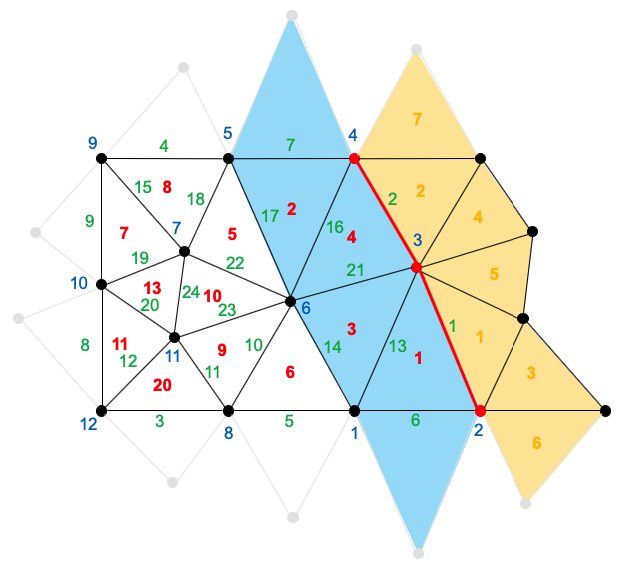
\includegraphics[height=3in]{Algorithm2.png}
   \caption{Illustration of nodal interpolation by the mesh in one of the partitions.}
   \label{figalg2}
\end{figure}

We have 12 nodes in this partition labeled blue. They are connected to cells via the cell-node
connectivity stored in the structure \verb+c2n+. Let's review the types of cells that connect to the
nodes:

\begin{enumerate}
   \item {\bf Interior cells}: labeled by red from 1 to 20. They are stored in the \verb+cells(:)+
      array.
   \item {\bf Partition (ghost) cells}: labeled by orange from 1 to 7. They are stored in the
      \verb+pcell(:)+ array in the structure \verb+itf+ (named as \verb+interf+).
   \item{\bf Boundary (ghost) cells}: there is no label. They are the \verb+right_cell+ of the
      boundary faces labeled from 3 to 9.
\end{enumerate}

All of the cells have the attributes \verb+c2n(:)+ that stores the indices of nodes (1 to 20) that
associated with the cell. Therefore, we can find the distance between any cell center to its
associated nodal coordinates. We add the \verb+weight+ attribute to the type \verb+cell+:

\begin{lstlisting}{language=[90]Fortran}
   type cell
      ...
      real, pointer :: weight(:)
   end type cell
\end{lstlisting}

The length of the \verb+weight+ will be equal to the length of the integer pointer \verb+c2n+. We
can assign the weights by:

\begin{lstlisting}{language=[90]Fortran}
   loop cells
      for each cell cc
      loop c2n of cc
         find node by nodes(cc(c2n(:)))
         for each node cn
         compute inverse distance between cc % centp to cn % xyz
         and save it to cc % weight
      end loop

      normalize cc % weight
   end loop

   looping parition cells, same
   looping boundary cells, same
\end{lstlisting}

and the nodal interpolation can be done by:

\begin{lstlisting}{language=[90]Fortran}
   nodes % qv = zero
   loop cells
      for each cell cc
      loop c2n of cc
         find node by nodes(cc(c2n(:)))
         for each node cn, get the weights for this node
         cn % qv = cn % qv + cc % qv * this weight 
      end loop
   end loop

   looping parition cells, same
   looping boundary cells, same
\end{lstlisting}

Once the nodal primitive variables $Q_{p,N}$ are computed, we can compute the face primitive
variables $Q_{p,i}$ (faces are labeled by green in Fig. \ref{figalg2}) by Eqn. \ref{eqf2n}, which
can be used to compute the cell gradient in Eqn. \ref{eqGreen}. Notice that $Q_{p,i}$ will also be
used when computing the viscous flux $F_{vn}$ in Eqn. \ref{eqlh1}. \paraspace

Now let's tackle the issue of the sign of the normal vector $n_{Ii}$. The face norm can be readily
computed knowing the nodal coordinates on the face. But the direction of this norm is still
depending. We mandate that the {\bf face norm} always points from its \verb+left_cell+ to its
\verb+right_cell+. This face norm is stored in the type \verb+face+, denoted as $n_i$. We add the
\verb+vecn+ attributes to the type \verb+face+ to store the face norm:

\begin{lstlisting}{language=[90]Fortran}
   type face
      ...
      real :: vecn(ndim)  ! ndim is number of dimensions
   end type face
\end{lstlisting}

We need not to separately store face norms $n_{Ii}$ for each cell $I$, as we already know $n_i$, and
$n_i$ and $n_{Ii}$ only differ by the sign. We note that when computing the gradient via Eqn.
\ref{eqGreen}, the gradient becomes a summation. We can elegantly deal with the sign of face norms
by choosing to loop over faces but not the cells, as follows:

\begin{lstlisting}{language=[90]Fortran}
   subroutine cell_gradient
      cells % gradient = zero
      loop faces
         for each face cf
         find the associated nodes by cf % f2n
         average nodal primitives as face primitives qvf
         cl => cf % left_cell
         cr => cf % right_cell
         a = cf % area
         
         loop i = 1, 2, 3
            cl % gradient(:,i) = cl % gradient(:,i) + 
                                 qvf * cf % vecn(i) * a
            cr % gradient(:,i) = cr % gradient(:,i) - 
                                 qvf * cf % vecn(i) * a
         end loop
      end loop
      cells % gradient = cells % gradient / cells % vol
   end subroutine cell_gradient
\end{lstlisting}

Note that for the \verb+left_cell+ we use the plus sign in the summation, but for the
\verb+right_cell+ we use the minus sign. This is because for the left cell, $n_i$ and $n_{Ii}$ have
the same sign, as $n_i$ points {\bf from left cell to right cell} and $n_{Ii}$ points {\bf out of
cell}. This is the opposite for the right cell. \paraspace

\subsubsection{Face Gradient}

At the last of this section, we discuss the computation of gradient of primitive variables at each
face $i$, which will be used in the computation of viscous flux $F_{vn}$ in Eqn. \ref{eqlh1}. We
take a similar approach as the LMS method in the cell gradient computation. First we compute for
each face $i$, three directional vectors as shown in Fig. \ref{figalg3}. This is illustrated in 3D
as an example, and in 2D, we only need to construct two directional vectors for each face $i$. The
first directional vector $d_{i1}$ always originates from the left cell (indexed as $il$) center and
ends at the right cell (indexed as $ir$) center. For the rest two directional vectors, if the face
is quadrilateral, $d_{i2}$ and $d_{i3}$ would be a ``cross'' connecting the diagonal nodes belonging
to face $i$. If the face is triangle, $d_{i2}$ and $d_{i3}$ are two edges of the triangle (randomly
chosen with random pointing directions).

\begin{figure}[H]
   \centering
   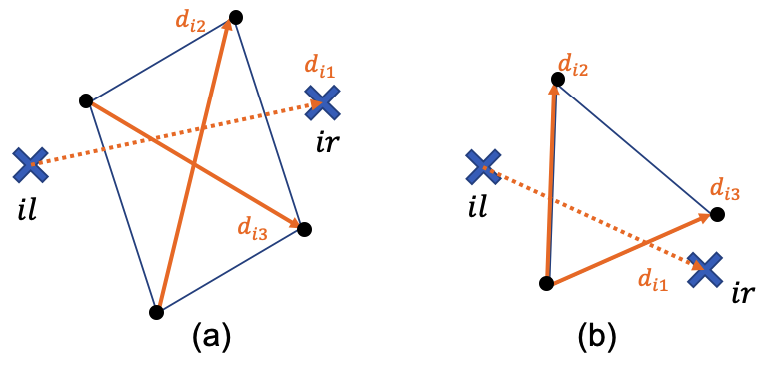
\includegraphics[height=2in]{Algorithm3.png}
   \caption{Illustration of face gradient computations. (a) Quadrilateral face and (b) Triangle
   face.}
   \label{figalg3}
\end{figure}

Now similar to Eqn. \ref{eqlms1}, we can write down the following approximation (again, take the
pressure gradient as an example):

\begin{align}\label{eqlmsface1}
   \begin{split}
      &\begin{bmatrix}
         \Delta x_{i1} & \Delta y_{i1} & \Delta z_{i1} \\
         \Delta x_{i2} & \Delta y_{i2} & \Delta z_{i2} \\
         \Delta x_{i3} & \Delta y_{i3} & \Delta z_{i3} \\
      \end{bmatrix} \begin{bmatrix}\partial_x p \\ \partial_y p \\ \partial_z p\end{bmatrix} \approx
      \begin{bmatrix}\Delta p_{i1} \\\Delta p_{i2} \\\Delta p_{i3} 
         \end{bmatrix} \\ &\textrm{where} \quad \begin{bmatrix}\Delta x_{ij} & \Delta y_{ij} &
      \Delta z_{ij}\end{bmatrix} = d_{ij}^T, j = 1,2,3
   \end{split}
\end{align}

Here the term $\Delta p_{ij}$ are taken to be the pressure difference between the starting and
ending point of the directional vectors. For example, $\Delta p_{i1} = p_{ir} - p_{il}$, etc. Note
that the nodal primitive variables should already been computed by the weighted inverse distance
average algorithm discussed previously. We note that Eqn. \ref{eqlmsface1} is not an over-determined
system and can be solved by a direct inversion:

\begin{align}\label{eqlmsface2}
   \begin{bmatrix}\partial_x p \\ \partial_y p \\ \partial_z p\end{bmatrix} = 
      \begin{bmatrix}
         \Delta x_{i1} & \Delta y_{i1} & \Delta z_{i1} \\
         \Delta x_{i2} & \Delta y_{i2} & \Delta z_{i2} \\
         \Delta x_{i3} & \Delta y_{i3} & \Delta z_{i3} \\
      \end{bmatrix}^{-1} \begin{bmatrix}\Delta p_{i1} \\\Delta p_{i2} \\\Delta p_{i3}\end{bmatrix}
\end{align}

We can further write the gradients for all the primitive variables as:

\begin{align}\label{eqlmsface3}
   \begin{bmatrix}\partial_x Q_p^T \\ \partial_y Q_p^T \\ \partial_z Q_p^T\end{bmatrix} = 
      \begin{bmatrix}
         a_{x1} & a_{x2} & a_{x3} \\
         a_{y1} & a_{y2} & a_{y3} \\
         a_{z1} & a_{z2} & a_{z3} \\
         \end{bmatrix} \begin{bmatrix}\Delta Q_{p,i1}^T \\\Delta Q_{p,i2}^T \\\Delta Q_{p,i3}^T\end{bmatrix}
\end{align}

Notice the similarity between Eqn. \ref{eqlmsface3} and Eqn. \ref{eqlms3} where the cell gradient
is computed. Here the matrix with elements $a$'s is exactly the matrix on the RHS of Eqn.
\ref{eqlmsface2} and can be understood as contributing weights just as the $s$ matrix in Eqn.
\ref{eqlms3}. For example, the element $a_{x1}$ indicates the contributing weight of $\Delta
Q_{p,i1}$ to the $x$ components of gradient, $\partial_x Q_p$. We shall precompute the $a$ matrix
and store it in the type \verb+face+ by the attributes \verb+avec+:

\begin{lstlisting}{language=[90]Fortran}
   type face
      ...
      real :: avec(ndim,ndim)
   end type face
\end{lstlisting}

By doing this, we only need to compute the matrix multiplication in Eqn. \ref{eqlmsface2} to obtain
the gradient at face $i$.

\clearpage
\section{Face Flux Computation}

With the gradient (cell and face) calculated as discussed in the previous section, we are ready to
the compute the convective flux $\F$ and viscous flux $F_{vn}$ in Eqn. \ref{eqexp1}. The convective
flux $\F$ is a function of the left and right state. We shall discuss in this section the
construction of the left and right states, and the expression of the flux function $\F$.  The
viscous flux $F_{vn}$ is a function of the face average primitive variables $Q_{p,i}$ and face
gradient $(\nabla \op Q_p)_i$. We have already calculated $Q_{p,i}$ as in Eqn. \ref{eqf2n} and
$(\nabla \op Q_p)_i$ as in Eqn. \ref{eqlmsface3}. Then we can substitute the variables into the
expression of $F_{vn}$ in Eqn. \ref{eqgovalg} to obtain the viscous flux.

\subsubsection{Construction of Left and Right States}

The concept left and right states originates from 1D Riemann problem \cite{toro2013riemann}. The
setup of the Riemann problem is as follows: assuming a discontinuity of primitive variables at $x =
0$, with $Q_p = Q_{pL}$ throughout the region of $x < 0$, and $Q_p = Q_{pR}$ throughout $x > 0$,
find the solution to the 1D conservation equation (similar to Eqn.  \ref{eq1DEuler}).
Specifically, find the (convective) flux at $x = 0$. We refer to $Q_{pL}$ and $Q_{pR}$ as the left
and right states for the 1D Riemann problem. \paraspace

The idea seems to be odd that the computation of flux function $\F$ can be relate to solving a 1D
Riemann problem. But it turns out this idea, credited to Godunov \cite{toro2013riemann}, is the
principal method of computing face flux $\F$. That is, for each face $i$, we formulate a 1D Riemann
problem along the face norm of $i$, and assuming the face center as the origin, we construct the
left and right states based on the left and right cells of face $i$ as the initial condition of the
1D Riemann problem. Then, we solve the 1D Riemann problem, whose analytical solution exists, and use
the flux across the origin as the flux $\F$ in Eqn. \ref{eqexp1}. This is referred to as the {\bf
Godunov's method} of flux calculation. There is generally two steps of this method: (1) to construct
the left and right states with some interpolation schemes and (2) solve the Riemann problem with the
exact analytical solution, or with an {\bf approximate Riemann solver}. \paraspace

Let's consider the configuration shown in Fig. \ref{figlrstates}. Face $i$ has left cell $I = il$
and right cell $J = il$. The green squares are the cell center and the two black circle shows the
location just on the left and right side of the face center. The orange vectors are pointing from
the left/right cells to the center of face $i$: $r_{Ii} = r_{il}$ and $r_{Ji} = r_{ir}$. A
simple-minded construction of left and right state would be to directly use the cell center values:

\begin{align*}
   Q_{p,iL} = Q_{p,il}, \quad Q_{p,iR} = Q_{p,ir}
\end{align*}

This is a {\bf first-order} approximation and is often not adequate for desired accuracy. A {\bf
second-order} approximation would be:

\begin{align*}
   Q_{p,iL} = Q_{p,il} + (\nabla \op Q_p)_{il} \cdot r_{il}, \quad Q_{p,iR} = Q_{p,ir} + (\nabla \op Q_p)_{ir} \cdot r_{ir}
\end{align*}

which is basically an interpolation with cell gradient of $I$ and $J$.

\begin{figure}[H]
   \centering
   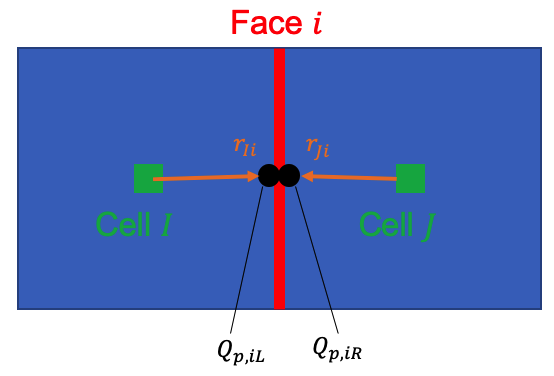
\includegraphics[height=2in]{Algorithm4.png}
   \caption{Construction of left and right states. 2D rectangle cells are used for illustration but
   the geometry can be generalized.}
   \label{figlrstates}
\end{figure}

The second-order approximation seems to be promising to ensure accuracy. However, the interpolation
can cause overshoot (or numerical oscillations) at sharp discontinuities like a shock wave.
Historically, this has been an infamous problem associated with Godunov's method (Godunov's curse).
Using first-order approximation leads to less accurate results, which typical manifests excessive
dissipation, while using second-order leads to numerical oscillations with sharp discontinuities
\cite{hirsch1988numerical}. The solution to Godunov's curse is the {\bf limiter}. Essentially, we
still apply second-order approximation but we revert back to first-order approximation whenever a
local extrema (maxima and minima), which tends to cause numerical oscillations, is detected. We
apply the {\bf limiter operator}, $\Psi$, when constructing the left/right states:

\begin{align}\label{eqlimiter}
   Q_{p,iL} = Q_{p,il} + \Psi_{il} [(\nabla \op Q_p)_{il} \cdot r_{il}], \quad Q_{p,iR} = Q_{p,ir} +
   \Psi_{ir} [(\nabla \op Q_p)_{ir} \cdot r_{ir}]
\end{align}

The limiter operator will multiply a coefficients on each component of the vector it operates on. 
These coefficients, $(\psi_p, \psi_u, \psi_v, \psi_w, \psi_T)$, are calculated based on each cell
$I$, and will be 0 if cell $I$ is a local extrema for $p$, or $u$, etc., while being 1 if cell $I$
is not a local extrema. For example, the coefficient for pressure, $\psi_p$, can be computed as the
following when the {\bf Barth's limiter} is applied:

\begin{align}\label{eqbarth}
   \begin{split}
      &\psi_p = \underset{j \in I_{sf}}{\textrm{min}} =
      \begin{cases}
         \ \textrm{min}(1, \frac{p_{I,max}-p_I}{\Delta_{p, Ij}}), &\textrm{if }\Delta_{p, Ij} > 0 \\
         \ \textrm{min}(1, \frac{p_{I,min}-p_I}{\Delta_{p, Ij}}), &\textrm{if }\Delta_{p, Ij} < 0 \\
         \ 1, &\textrm{if }\Delta_{p, Ij} = 0 
      \end{cases} \\
      &\textrm{where }  \Delta_{p, Ij} = (\nabla p)_I \cdot r_{Ij}
   \end{split}
\end{align}

Here, $p_{I,max}$ and $p_{I,min}$ are the maximum and minimum pressure among cell $I$ and all of its
surrounding cells. Let's examine how Eqn. \ref{eqbarth} can achieve the function of a limiter.
Assume the pressure is increasing from cell $I$ towards one of its surrounding faces $j$, such
that $\Delta_{p,Ij} > 0$. In this case we expect the left/right state of face $j$ to have a larger
pressure $p$ than the cell $I$. Then, if $p_I$ is a {\bf not} a local maximum, the difference
$p_{I,max} - p_I$ should be larger than $\Delta_{p,Ij}$, and the limiter coefficient $\psi_p$ is
just 1. However, if $p_I$ is a local maximum, we do not want the left/right states to be constructed
to have even larger $p$. Therefore, the limiter coefficient $\psi_p$ is set to be 0, and we revert
back to a first-order approximation. We can see that the limiter makes the constructed left/right
states at faces not exceed the local extrema, and therefore, mitigate the overshoot/numerical
oscillation issue. We apply the similar formulation in Eqn. \ref{eqbarth} to compute the limiter
coefficients for $u$, $v$, $w$ and $T$, and we multiply these coefficients in Eqn. \ref{eqlimiter}
to construct the left/right states.

\subsubsection{Roe's Approximate Riemann Solver}

With the left and right states constructed with respect to face $i$, we formulate a pseudo 1D Riemann
problem along the face norm of $i$, as follows:

\begin{align}\label{eqpseudoRP}
   \Gamma \frac{\partial }{\partial t} \begin{bmatrix}p \\ u \\ v \\ w \\ T\end{bmatrix}+
   \frac{\partial }{\partial n} \begin{bmatrix}\rho V_{n,i} \\ \rho u V_{n,i} + p n_{i,x} \\ \rho v
   V_{n,i} + p n_{i,y} \\ \rho w V_{n,i} + p n_{i,z} \\ \rho h_{tot}V_{n,i} \end{bmatrix} = 0
\end{align}

where $n_i = (n_{i,x}, n_{i,y}, n_{i,z})$ is the face norm of face $i$, pointing from left cell to
right cell. $V_{n,i} = V \cdot n_i$ is the velocity along $n_i$. Eqn. \ref{eqpseudoRP} is
formulated based on the differential form of governing equation Eqn. \ref{eqmatgovDf} neglecting
viscous flux and source term, as well as assuming that the primitive variables only vary along the
$n_i$ direction, i.e.:

\begin{align*}
   \frac{\partial }{\partial x} = n_{ix} \frac{\partial }{\partial n}, \; 
   \frac{\partial }{\partial y} = n_{iy} \frac{\partial }{\partial n}, \;
   \frac{\partial }{\partial z} = n_{iz} \frac{\partial }{\partial n}
\end{align*}

We also point out that Eqn. \ref{eqpseudoRP} is formulated along the face norm $n_i$, which is
different from the direction of $n_{Ii}$ in Eqn. \ref{eqexp1} for the flux function $\F$. However,
as we will see later, this can be handled elegantly by a face-loop with careful sign considerations.
\paraspace

Now let's focus on solving Eqn. \ref{eqpseudoRP}. We can rewrite it as:

\begin{align*}
   \Gamma(Q_p) \frac{\partial Q_p}{\partial t} + \frac{\partial F_{cn}(Q_p)}{\partial n} = 0
\end{align*}

Note that $F_{cn}$ is solely a function of $Q_p$ as $n_i$ is a constant. With this, we take the
derivatives of $F_{cn}$ with respect to $Q_p$ to write:

\begin{align}\label{eqpseudoRPP1}
   \Gamma(Q_p) \frac{\partial Q_p}{\partial t} + A_{cn}(Q_p)\frac{\partial Q_p}{\partial n} = 0
\end{align}

Let's expand to see the expression for the two jacobians, i.e., the primitive jacobian $\Gamma$ and
the convective flux jacobian $A_{cn}$:

\begin{align}\label{eqGamma3D}
   \Gamma = 
   \begin{bmatrix}
      \rho_p & 0 & 0 & 0 & \rho_T \\
      \rho_p u & \rho & 0 & 0 & \rho_T u \\ 
      \rho_p v & 0 & \rho & 0 & \rho_T v \\
      \rho_p w & 0 & 0 & \rho & \rho_T w \\
      \rho_p h_{tot} - (1 - \rho h_p) & \rho u & \rho v & \rho w & \rho_T h_{tot} + \rho h_T
   \end{bmatrix}
\end{align}

and \paraspace

\begin{align}\label{eqAcn}
   \begin{split}
      &A_{cn} = \\
      &\begin{bmatrix}
         \rho_p V_n & \rho n_x & \rho n_y & \rho n_z & \rho_T V_n \\
         \rho_p u V_n + n_x & \rho u n_x + \rho V_n & \rho u n_y & \rho u n_z & \rho_T u V_n \\
         \rho_p v V_n + n_y & \rho v n_x & \rho v n_y + \rho V_n & \rho v n_Z & \rho_T v V_n \\
         \rho_p w V_n + n_z & \rho w n_x & \rho w n_y & \rho w n_z + \rho V_n & \rho_T w V_n \\
         (\rho_p h_{tot} + \rho h_p) V_n & \rho(u V_n + h_{tot}n_x) & \rho(v V_n + h_{tot}n_y) & \rho(w
         V_n + h_{tot}n_z) & (\rho_T h_{tot} + \rho h_T)V_n
      \end{bmatrix}
   \end{split}
\end{align}

where we dropped the subscript $i$ for the face index to indicate generality. Notice the similarity
between Eqn. \ref{eqpseudoRPP1} and Eqn. \ref{eq1DEulerP1}. We can understand Eqn.
\ref{eqpseudoRPP1} as 1D conservation equations with 5 conservative variables. Again, we can write
Eqn. \ref{eqpseudoRPP1} in a wave-equation form:

\begin{align}\label{eqpseudoRPP2}
   \frac{\partial Q_p}{\partial t} + \Gamma^{-1} A_{cn} \frac{\partial Q_p}{\partial n} = 0
\end{align}

Now our task is to solve Eqn. \ref{eqpseudoRPP2} given the initial condition of the left/right
state $(Q_{pL}, Q_{pR})$ and specifically, the solved flux across the origin will be taken as the
flux function $\F$. Although it is possible to solve Eqn. \ref{eqpseudoRPP2} analytically, such
effort costs too much computation time and in practice, an approximate Riemann solver is always
used. Here, we introduce {\bf Roe's Riemann solver} which is arguably the most popular Riemann
solver. \paraspace

The key idea of Roe's solver is to treat the system matrix $\Gamma^{-1} A_{cn}$ as a constant. This
constant matrix is first computed using the {\bf Roe's average} of primitive variables
$\tilde{Q_p}$, expressed as:

\begin{align}\label{eqRoeave}
   \begin{split}
      &\tilde{\rho} = \sqrt{\rho_L \rho_R} \\
      &\tilde{u} = \frac{u_L \sqrt{\rho_L} + u_R \sqrt{\rho_R}}{\sqrt{\rho_L} + \sqrt{\rho_R}} \\
      &\tilde{v} = \frac{v_L \sqrt{\rho_L} + v_R \sqrt{\rho_R}}{\sqrt{\rho_L} + \sqrt{\rho_R}} \\
      &\tilde{w} = \frac{w_L \sqrt{\rho_L} + w_R \sqrt{\rho_R}}{\sqrt{\rho_L} + \sqrt{\rho_R}} \\
      &\tilde{h} = \frac{h_L \sqrt{\rho_L} + h_R \sqrt{\rho_R}}{\sqrt{\rho_L} + \sqrt{\rho_R}} 
   \end{split}
\end{align}

Note that the Roe's average are expressed in the variables $(\rho,u,v,w,h)$ instead of our primitive
variables $(p,u,v,w,T)$. We typically adjust the Roe's average of $(\tilde{p}, \tilde{u}, \tilde{v},
\tilde{w}, \tilde{T})$, such that Eqn. \ref{eqRoeave} can be satisfied. We then plug the Roe's
averaged primitive variables $\tilde{Q_p}$ into Eqn. \ref{eqGamma3D} and \ref{eqAcn} to calculate
the system matrix $\Gamma^{-1} A_{cn}$. \paraspace

With the system matrix determined, Eqn. \ref{eqpseudoRPP2} becomes a system of linear wave
equations. We point out that with linear equations, the jacobian matrices are constant, and
therefore, we can transform between variables by simply multiplying a constant matrix. Specifically:

\begin{subequations}\label{eqjacobtrans}
   \begin{align}
   &F_{cn}(Q_p) = A_{cn}(\tilde{Q_p}) Q_p \\
   &Q_p = M(\tilde{Q_p}) \widehat{Q}
   \end{align}
\end{subequations}

where the diagonalization of the system matrix is expressed as: $\Gamma^{-1} A_{cn} = M \Lambda
M^{-1}$. As when transforming Eqn. \ref{eq1DEulerP2} to Eqn. \ref{eq1DEulerCh}, $\Lambda$ is a
diagonal matrix containing the eigenvalues of $\Gamma^{-1} A_{cn}$, $M$'s column vectors are the
eigenvectors of $\Gamma^{-1} A_{cn}$, and $\widehat{Q}$ is the characteristic variable. We emphasize
that the matrices $\Gamma$, $A_{cn}$, $M$, and $\Lambda$ are all treated as constant matrices when
solving Eqn.  \ref{eqpseudoRPP1} or \ref{eqpseudoRPP2}. These matrices are precomputed using the
Roe's average in Eqn. \ref{eqRoeave}. \paraspace

The roadmap of finding the analytical solution, denoted as $\Qcal_p$, of Eqn. \ref{eqpseudoRPP2} is as
follows:

\begin{enumerate}
   \item Transform the primitive variables to characteristic variables with Eqn. \ref{eqjacobtrans}b.
   \item Find the analytical solution of characteristic variables $\widehat{\Qcal}$ specifically at
      $n = 0$.
   \item Transform back to obtain $\Qcal_p$ at $n = 0$.
   \item Use Eqn. \ref{eqjacobtrans}a to find the flux at $n = 0$ and let it be the flux function
      $\F$.
\end{enumerate}                                               

Let's start with the first step, we can express the linear wave equations by the characteristic
variables as:

\begin{align}\label{eqChari}
   \frac{\partial \qh_i}{\partial t} + \lambda_i \frac{\partial \qh_i}{\partial n} = 0, \; i = 1, 2,
   \cdots 5
\end{align}

where $\qh_i$'s are the components of the characteristic variables $\Qh$ and $\lambda_i$'s are the
eigenvalues of the system matrix. Note that the equations for $i = 1, 2, \cdots 5$ are independent
with each other in Eqn. \ref{eqChari}. The structure of the analytical solutions can be represented
by the $n-t$ diagram shown in Fig. \ref{figNTDiag}. Each blue line in Fig. \ref{figNTDiag} is
referred to as a {\bf characteristic line} and is associated with a wave speed $\lambda_i$ ($i =
1, 2, \cdots, 5$), corresponding to the eigenvalues in Eqn. \ref{eqChari}. Each characteristic line
represents the solution of the $i^{th}$ equation for Eqn. \ref{eqChari}. For the $i^{th}$
characteristic line, the solution at any position $n$ and time $t$ is equal to the initial left
data, $\qh_{iL}$, if the point $(n,t)$ is situated at the left side of the characteristic line, and
the solution is equal to the initial right data $\qh_{iR}$, if $(n,t)$ is situated at the right side
of the characteristic line. Therefore, we can write the analytical solution for the characteristic
variables as:

\begin{align*}
   \widehat{q}_i = \begin{cases}
      \ \qh_{iL}, \; \textrm{if } n - \lambda_i t < 0 \\
      \ \qh_{iR}, \; \textrm{if } n - \lambda_i t > 0
   \end{cases}
\end{align*}

When making $n = 0$, the solution can be written as:

\begin{align*}
   \widehat{q}_i = \begin{cases}
      \ \qh_{iL}, \; \lambda_i < 0 \\
      \ \qh_{iR}, \; \lambda_i > 0
   \end{cases}
\end{align*}

Then, we can transform back to primitive variables by multiplying the solution for characteristic
variables with $M$. 

\begin{align}\label{eqAnl1}
   \Qcal_p = M\widehat{\Qcal} = \sum_i \qh_i m_i = \sum_{\lambda_i < 0} \qh_{iR} m_i +
   \sum_{\lambda_i > 0} \qh_{iL} m_i
\end{align}

where $m_i$'s are the column vectors of $M$ and are also the eigenvectors of the system matrix.

\begin{figure}[H]
   \centering
   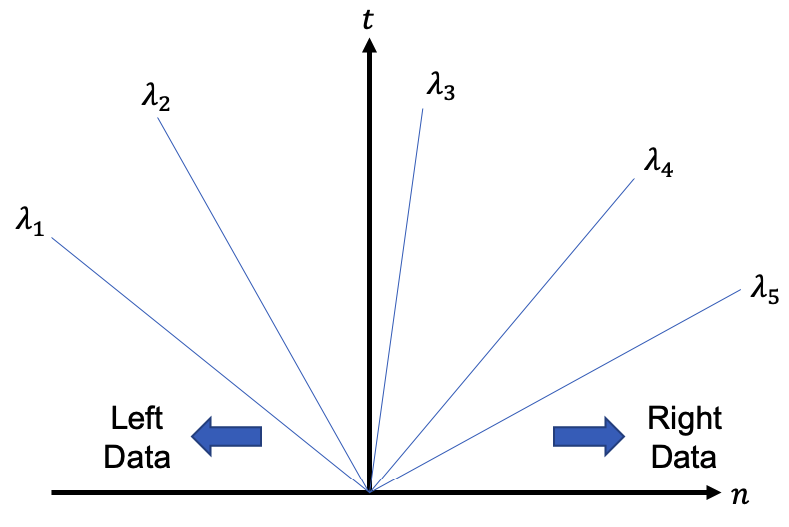
\includegraphics[height=3in]{Algorithm5.png}
   \caption{$n-t$ Diagram of the solution structure for a system of linear wave equation. 5
      characteristic lines are shown for the system in Eqn. \ref{eqpseudoRPP2}. For
   convenience of discussion, we assume $\lambda_1 < \lambda_2 < \cdots < \lambda_5$.}
   \label{figNTDiag}
\end{figure}

With some algebraic manipulation, Eqn. \ref{eqAnl1} can be written as:

\begin{align}\label{eqAnl2}
   \begin{split}
      &\Qcal_p = \frac{1}{2}(Q_{pL} + Q_{pR}) - \frac{1}{2} \sum_i \textrm{sgn}(\lambda_i) (\qh_{iR}
      - \qh_{iL}) m_i \\
      &\textrm{Note:  } Q_{pL} = \sum_i \qh_{iL} m_i, \; Q_{pR} = \sum_i \qh_{iR} m_i
   \end{split}
\end{align}

where we sgn function is $+1$ when $\lambda_i$ is positive and $-1$ when $\lambda_i$ is
negative. Finally, we multiply $A_{cn}$ with $\Qcal_p$ in Eqn. \ref{eqAnl2} to obtain the flux
function $\F$:

\begin{align}\label{eqFlux1}
   \F = A_{cn} \Qcal_p = \frac{1}{2}(F_{cn}(Q_{pL}) + F_{cn}(Q_{pR})) - \frac{1}{2}A_{cn} \sum_i
   \textrm{sgn}(\lambda_i) \Delta \qh_i m_i
\end{align}

where $\Delta \qh_i = \qh_{iR} - \qh_{iL}$ and we have applied Eqn. \ref{eqjacobtrans}a as a
linearization approximation. We can further simplify Eqn. \ref{eqFlux1} by realizing $A_{cn} =
\Gamma \Gamma^{-1} A_{cn}$ and $\Gamma^{-1} A_{cn} m_i = \lambda_i m_i$. Therefore:

\begin{align*}
   A_{cn}\sum_i \textrm{sgn}(\lambda_i) \Delta \qh_i m_i &= \Gamma \Gamma^{-1} A_{cn} \sum_i
   \textrm{sgn}(\lambda_i) \Delta \qh_i m_i \\
   &= \Gamma \sum_i \textrm{sgn}(\lambda_i) \Delta \qh_i \Gamma^{-1} A_{cn} m_i \\
   &= \Gamma \sum_i \textrm{sgn}(\lambda_i) \lambda_i \Delta \qh_i m_i \\
   &= \Gamma \sum_i |\lambda_i| \Delta \qh_i m_i \\
   &= \Gamma M |\Lambda| \Delta \Qh
\end{align*}

where $\Lambda = \textrm{diag}\{|\lambda_1|, |\lambda_2|, \cdots, |\lambda_5|\}$ and $\Delta \Qh =
\Qh_R - \Qh_L$. Finally, we apply $\Delta \Qh = M^{-1}(Q_{pR} - Q_{pL})$ to obtain:

\begin{align}\label{eqFlux2}
   \F = \frac{1}{2}(F_{cn}(Q_{pL}) + F_{cn}(Q_{pR})) - \frac{1}{2}\Gamma M |\Lambda| M^{-1} (Q_{pR}
   - Q_{pL})
\end{align}

Since $\Gamma^{-1}A_{cn} = M \Lambda M^{-1}$, we sometimes make the notation $|\Gamma^{-1}A_{cn}| =
M |\Lambda| M^{-1}$, which makes the Eqn. \ref{eqFlux2} be written as \cite{li2006unified}:

\begin{align}\label{eqFlux3}
   \F = \frac{1}{2}(F_{cn}(Q_{pL}) + F_{cn}(Q_{pR})) - \frac{1}{2}\Gamma |\Gamma^{-1}A_{cn}| (Q_{pR}
   - Q_{pL})
\end{align}

Eqn. \ref{eqFlux3} is the definitive expression of the flux funciton. We can find that the flux
funciton is composed of two parts on the RHS of Eqn. \ref{eqFlux3}. The first part is simply an
average of the convective flux $F_{cn}$ (Eqn. \ref{eqpseudoRP}) with the left and right states. The
second part is an {\bf artifial dissipation} which resists the flux from left to right cell and is
proportional to the difference between the right and left states $(Q_{pR} -  Q_{pL})$. The artifial
dissipation is used to improve the stability of the numerical scheme and it will diminish as the
mesh size decreases ($Q_{pR} -  Q_{pL}$ decreases). We can write the flux function generally as:

\begin{align}\label{eqFluxAD}
   \F = \frac{1}{2}(F_{cn}(Q_{pL}) + F_{cn}(Q_{pR})) - \frac{1}{2}A_D (Q_{pR}
   - Q_{pL})
\end{align}

where the matrix $A_D$ represents the amount of artifial dissipation in the flux function.
\paraspace

To summarize the computation of $\F$, we first compute the convective part of Eqn. \ref{eqFlux3}
with the contructed left and right states. Then we calculate the Roe's average of the left and right
states $\tilde{Q}_p$ using Eqn. \ref{eqRoeave}. Finally, the artifial dissipation matrix
$A_D = \Gamma M |\Lambda| M^{-1}$can be computed using $\tilde{Q}_p$. In computing the
artifial dissipation matrix, we will be using Eqn. \ref{eqGamma3D} and \ref{eqAcn}. Notice that
in these expression, the derivatives $\rho_p$, $\rho_T$, $h_p$, $h_T$, etc. are still functions of
the primitive variables. Therefore, all the terms related to $A_D$ can be computed based
on the Roe's average $\tilde{Q}_p$.

\subsubsection{Some Computational Details of Viscous Flux}

The viscous flux at each face $i$ is computed with the expression given in Eqn. \ref{eqgovalg},
which can expanded as:

\begin{align}\label{eqFvnexpand}
   F_{vn} = \begin{bmatrix}0 \\ \tau \cdot n \\ (\tau^T \cdot V - q) \cdot n\end{bmatrix} = \begin{bmatrix}
      0 & 0 & 0 \\
      \tau_{xx} & \tau_{xy} & \tau_{xz} \\
      \tau_{yx} & \tau_{yy} & \tau_{yz} \\
      \tau_{zx} & \tau_{zy} & \tau_{zz} \\
      E_x & E_y & E_z
      \end{bmatrix} \begin{bmatrix}n_x \\ n_y \\ n_z\end{bmatrix}
\end{align}

where $(n_x, n_y, n_z)$ is the face norm. We have dropped the face index $i$ to indicate generality.
The vector $(E_x, E_y, E_z)^T$ is expressed as:

\begin{align}\label{eqFvnEng}
   \begin{bmatrix} E_x \\ E_y \\ E_z\end{bmatrix} = 
   \begin{bmatrix}
      \tau_{xx} & \tau_{xy} & \tau_{xz} \\
      \tau_{yx} & \tau_{yy} & \tau_{yz} \\
      \tau_{zx} & \tau_{zy} & \tau_{zz}
      \end{bmatrix} \begin{bmatrix}u \\ v \\ w\end{bmatrix} + k \begin{bmatrix} \partial_x T \\
   \partial_y T \\ \partial_z T\end{bmatrix}
\end{align}

Note that $(E_x, E_y, E_z)^T$ comes from the work done by the viscous stress and the conductive heat
flux $q = k\nabla T$. The expression for the viscous stress tensor $\tau$ can be found in Eqn.
\ref{eqviscousstress}. It is noted that the rows of $F_{vn}$ related to momentum (row 2, 3 and 4)
are only dependent on the face gradient, which is calculated by Eqn. \ref{eqlmsface3}. Row 5 of
$F_{vn}$ relates to energy and is dependent on both the face gradient and the velocity $(u, v, w)$
on the face, as indicated by Eqn. \ref{eqFvnEng}. These velocities will be calculated as the nodal
averages given in Eqn. \ref{eqf2n}. \paraspace

It is useful in the implementation of the computation of Eqn. \ref{eqFvnexpand} to express $F_{vn}$
as some matrix multiplications with the gradient vectors $\partial_x Q_p$, $\partial_y Q_p$ and
$\partial_z Q_p$. We can manipulate the expression in Eqn. \ref{eqFvnexpand} as:

\begin{align}\label{eqFvnRij}
   \begin{split}
      &F_{vn} = \begin{bmatrix}F_{vn,x} & F_{vn,y} & F_{vn,z}\end{bmatrix}
      \begin{bmatrix}n_x \\ n_y \\ n_z\end{bmatrix}, \; \textrm{where} \\
      &F_{vn,x} = \begin{bmatrix}0 & \tau_{xx} & \tau_{yx} &\tau_{zx} & E_x\end{bmatrix}^T =
      R_{xx}\partial_x Q_p + R_{xy}\partial_y Q_p + R_{xz} \partial_z Q_p \\
      &F_{vn,y} = \begin{bmatrix}0 & \tau_{xy} & \tau_{yy} &\tau_{zy} & E_y\end{bmatrix}^T =
      R_{yx}\partial_x Q_p + R_{yy}\partial_y Q_p + R_{yz} \partial_z Q_p \\
      &F_{vn,z} = \begin{bmatrix}0 & \tau_{zx} & \tau_{zy} &\tau_{zz} & E_z\end{bmatrix}^T =
      R_{zx}\partial_x Q_p + R_{zy}\partial_y Q_p + R_{zz} \partial_z Q_p \\
   \end{split}
\end{align}

The matrices $R_{ij}$ ($i = x, y, z$ and $j = x, y, z$) are referred to as the {\bf viscous
matrices} and will be listed later. We note that the gradients of $Q_p$ are evaluated at each face
$i$ and can be viewed as the following linear combinations:

\begin{align}\label{eqGradLinear}
   \begin{split}
      (\partial_x Q_p)_i = \sum_{j = 1}^3 a_{xj} \Delta Q_{p,ij} \\
      (\partial_y Q_p)_i = \sum_{j = 1}^3 a_{yj} \Delta Q_{p,ij} \\
      (\partial_z Q_p)_i = \sum_{j = 1}^3 a_{zj} \Delta Q_{p,ij}
   \end{split}
\end{align}

For each face $i$, the face gradient is contributed from three components, each of which is a
difference of primitive variables surrounding face $i$. For example, $\Delta Q_{p,i1} = Q_{p,ir} -
Q_{p,il}$ (Fig. \ref{figalg3}). The coefficients $a_{ij}$ with $i = x, y, z$ and $j = 1, 2, 3$ comes
from the matrix inversion in Eqn. \ref{eqlmsface2} and are the $a_{ij}$'s expressed in Eqn.
\ref{eqlmsface3}. \paraspace

We list the expressions for the viscous matrices:

\begin{align}\label{eqVisMat}
   \begin{split}
      &R_{xx} = \begin{bmatrix}
         0 & 0 & 0 & 0 & 0 \\
         0 & \frac{4}{3}\mu & 0 & 0 & 0 \\
         0 & 0 & \mu & 0 & 0 \\
         0 & 0 & 0 & \mu & 0 \\
         0 & \frac{4}{3}\mu u & \mu v & \mu w & k
      \end{bmatrix} \,
      R_{xy} = \begin{bmatrix}
         0 & 0 & 0 & 0 & 0 \\
         0 & 0 & -\frac{2}{3}\mu & 0 & 0 \\
         0 & \mu & 0 & 0 & 0 \\
         0 & 0 & 0 & 0 & 0 \\
         0 & \mu v & -\frac{2}{3}\mu u & 0 & 0
      \end{bmatrix} \,
      R_{xz} = \begin{bmatrix}
         0 & 0 & 0 & 0 & 0 \\
         0 & 0 & 0 & -\frac{2}{3}\mu & 0 \\
         0 & 0 & 0 & 0 & 0 \\
         0 & \mu & 0 & 0 & 0 \\
         0 & \mu w & 0 & -\frac{2}{3}\mu u& 0
      \end{bmatrix} \\[10pt]
      &R_{yx} = \begin{bmatrix}
         0 & 0 & 0 & 0 & 0 \\
         0 & 0 & \mu & 0 & 0 \\
         0 & -\frac{2}{3}\mu & 0 & 0 & 0 \\
         0 & 0 & 0 & 0 & 0 \\
         0 & -\frac{2}{3}\mu v & \mu u & 0 & 0
      \end{bmatrix} \,
      R_{yy} = \begin{bmatrix}
         0 & 0 & 0 & 0 & 0 \\
         0 & \mu & 0 & 0 & 0 \\
         0 & 0 & \frac{4}{3}\mu & 0 & 0 \\
         0 & 0 & 0 & \mu & 0 \\
         0 & \mu u & \frac{4}{3}\mu v & \mu w & k
      \end{bmatrix} \,
      R_{yz} = \begin{bmatrix}
         0 & 0 & 0 & 0 & 0 \\
         0 & 0 & 0 & 0 & 0 \\
         0 & 0 & 0 & -\frac{2}{3}\mu & 0 \\
         0 & 0 & \mu & 0 & 0 \\
         0 & 0 & \mu w & -\frac{2}{3}\mu v& 0
      \end{bmatrix}\\[10pt]
      &R_{zx} = \begin{bmatrix}
         0 & 0 & 0 & 0 & 0 \\
         0 & 0 & 0 & \mu & 0 \\
         0 & 0 & 0 & 0 & 0 \\
         0 & -\frac{2}{3}\mu & 0 & 0 & 0 \\
         0 & -\frac{2}{3}\mu w & 0 & \mu u & 0
      \end{bmatrix} \,
      R_{zy} = \begin{bmatrix}
         0 & 0 & 0 & 0 & 0 \\
         0 & 0 & 0 & 0 & 0 \\
         0 & 0 & 0 & \mu & 0 \\
         0 & 0 & -\frac{2}{3}\mu & 0 & 0 \\
         0 & 0 & -\frac{2}{3}\mu w & \mu v & 0
      \end{bmatrix}
      R_{zz} = \begin{bmatrix}
         0 & 0 & 0 & 0 & 0 \\
         0 & \mu & 0 & 0 & 0 \\
         0 & 0 & \mu & 0 & 0 \\
         0 & 0 & 0 & \frac{4}{3}\mu & 0 \\
         0 & \mu u & \mu v & \frac{4}{3}\mu w & k
      \end{bmatrix}
   \end{split}
\end{align}

To summarize, we first compute the face gradient with the linear combinations in Eqn.
\ref{eqGradLinear}, and then evaluate the viscous matrices in Eqn. \ref{eqVisMat}. Note that in
viscous matrices, the viscosity $\mu$ and thermal conductivity $k$ can be functions of primitive
variables. We can use the nodal averaged $Q_p$ at face to evaluate $\mu$ and $k$. Alternately, we
can first evaluate $\mu$ and $k$ at the left and right cell with the cell primitive variables, and
then take the average to be the $\mu$ and $k$ at the face for the viscous matrices in Eqn.
\ref{eqVisMat}. For the velocities $(u, v, w)$ in viscous matrices, we always use the nodal averaged
values.

\subsubsection{Face Loop for Assigning Fluxes to Cells}

To close this section, we discuss the assignment of face fluxes to the \verb+res+ attribute for each
\verb+cell+. As we see in Eqn. \ref{eqlh1}, for each cell $I$, the convective flux $\F$ and viscous
flux $F_{vn}$ are summed over cell $I$'s surrounding faces. This summation is then added to the
residual of cell $I$, $\R_I$. In practical implementation, we do not need to loop over the cell
array \verb+cells(:)+ and sum over the surrounding faces for each cell. Instead, we can loop over the
face array \verb+faces(:)+ and assign the face flux to the corresponding left and right cells. An
outline of the computation is as follows:


\begin{lstlisting}{language=[90]Fortran}
   subroutine convective_flux
      loop faces
         for each face cf
         cl => cf % left_cell
         cr => cf % right_cell

         ! left and right states have been constructed
         calculate the convective flux as faceflux

         cl % res = cl % res - faceflux 
         cr % res = cr % res + faceflux
      end loop
   end subroutine convective_flux

   subroutine viscous_flux
      loop faces
         for each face cf
         cl => cf % left_cell
         cr => cf % right_cell

         ! face primitive variables and gradients have been calculated
         calculate the viscous flux as faceflux

         cl % res = cl % res + faceflux 
         cr % res = cr % res - faceflux
      end loop
   end subroutine viscous_flux
\end{lstlisting}

Let's examine the sign of \verb+faceflux+ when assigning to the left and right cells. When
calculating fluxes (convective or viscous) for face $i$, the face norm $n_i$ is always pointing from
the left cell to the right cell. Therefore, the flux has the correct sign for the left cell ($n_i$
points {\bf out of} left cell and aligns with $n_{Ii}$ in Eqn. \ref{eqlh1}).  The flux will have the
opposite sign for the right cell ($n_i$ points {\bf into} the right cell and has the opposite sign
with $n_{Ii}$). However, we notice that there is a minus sign in the residual $\R_I$ in Eqn.
\ref{eqlh1}. Also, in the summation over $I_{sf}$, the convective flux $\F$ has the plus sign while
the viscous flux $F_{vn}$ has the minus sign. Taking all this into account, we can conclude that for
convective flux, \verb+cl % res+ must subtract the \verb+faceflux+, and \verb+cr % res+ must add up
the \verb+faceflux+. However, for viscous flux, the opposite should be done: \verb+cl % res+ must
add up the \verb+faceflux+ and \verb+cr % res+ must subtract the \verb+faceflux+.
\paraspace


\clearpage
\section{Implicit Temporal Discretization}

In this section, let's consider an alternative way of temporal discretization. Let's examine Eqn.
\ref{eqexp1}: the first term in the LHS is the temporal evolution of primitive/conservative
variables. The second and third term are the convective and viscous flux, evaluated at time step
$n$. The RHS is the source term evaluated at time step $n$. We note that the primitive variable at
the next time step $n+1$ can be directly updated with the convective flux, viscous flux and source
term evaluated at time step $n$. This is referred to as the explicit temporal discretization. In the
{\bf implicit temporal discretization}, the above-mentioned terms are evaluated at time step $n+1$,
which can be expressed as:

\begin{align}\label{eqimpExpand}
   \begin{split}
      \Gamma(Q_{p,I}^n) \frac{2Q_{p,I}^{n+1} - 3Q_{p,I}^n + Q_{p,I}^{n-1}}{2\Delta t} \Omega_I +
      &\sum_{i \in I_{sf}} \F(Q_{pL,i}^{n+1}, Q_{pR,i}^{n+1}, n_{Ii}) \sigma_i - \\ &\sum_{i \in
      I_{sf}} F_{vn}(Q_{p,i}^{n+1}, (\nabla \mathop{\otimes} Q_p)_i^{n+1}, n_{Ii}) \sigma_i =
      S(Q_{p,I}^{n+1})
      \Omega_I
   \end{split}
\end{align}

We use the {\bf linearization} to approximate the terms in time step $n+1$:

\begin{align}\label{eqlinapp}
   \begin{split}
      &\F^{n+1} \approx \F^n + \left(\frac{\partial \F}{\partial
      Q_{pl,i}}\right)^n \Delta Q_{pl,i}^n + \left(\frac{\partial \F}{\partial Q_{pr,i}}\right)^n \Delta
      Q_{pr,i}^n \\ & F_{vn}^{n+1} \approx F_{vn}^n + \left(\frac{\partial F_{vn}}{\partial
      Q_{pl,i}}\right)^n \Delta Q_{pl,i}^n +
      \left(\frac{\partial F_{vn}}{\partial Q_{pr,i}}\right)^n \Delta Q_{pr,i}^n \\ & S^{n+1}
      \approx S^n + \left(\frac{\partial S}{\partial Q_{p,I}}\right)^n \Delta Q_{p,I}^n
      \\ &\textrm{where } \Delta Q_{pl,i}^n = Q_{pl,i}^{n+1} - Q_{pl,i}^n, \; \Delta Q_{pr,i}^n =
      Q_{pr,i}^{n+1} - Q_{pr,i}^n, \; \textrm{and } \Delta Q_{p,I}^n = Q_{p,I}^{n+1} - Q_{p,I}^n
   \end{split}
\end{align}

In Eqn. \ref{eqlinapp}, $\F^n$, $F_{vn}^n$ and $S^n$ are still evaluated with the corresponding
terms at time step $n$ as in Eqn. \ref{eqexp1}. The terms with Jacobian matrices can be understood
as the first-order terms from a Taylor series expansion. $\F$, $F_{vn}$ are viewed as functions of
$Q_{pl,i}$ and $Q_{pr,i}$ (primitive variables from the left and right cells of face $i$). $S$ is
viewed as a function of $Q_{p,I}$ (primitive variables of cell $I$). We note that technically, $\F$
is a function of the left and right states, and $F_{vn}$ is a function of the face primitive
variable and its gradient. However, Eqn. \ref{eqlinapp} is only a ``first-order'' approximation.
Indeed, $\F$ and $F_{vn}$ should be related to more cells surrounding face $i$ besides only the left
and right cells of face $i$. Theoretically, there can be higher-order terms on the RHS of Eqn.
\ref{eqlinapp}, but as we will discuss later, the approximation of Eqn. \ref{eqlinapp} needs not be
meticulously accurate, and the first-order approximation is found adequate in practice.
\paraspace

Now let's make the following notations on the jacobian matrices:

\begin{align}\label{eqfacejacob}
   \begin{split}
      &\F^{n+1} \approx \F^n + A_{cl,i}^n \Delta Q_{pl,i}^n + A_{cr,i}^n \Delta Q_{pr,i}^n \\
      &F_{vn}^{n+1} \approx F_{vn}^n + A_{vl,i}^n \Delta Q_{pl,i}^n + A_{vr,i}^n \Delta Q_{pr,i}^n \\
      &S^{n+1} = S^n + A_{S,I}^n \Delta Q_{p,I}^n
   \end{split}
\end{align}

The computation of the matrices $A_{cl,i}^n$, $A_{cr,i}^n$, $A_{vl,i}^n$, $A_{vr,i}^n$ and
$A_{S,I}^n$ will be detailed later. Now, substitute Eqn. \ref{eqfacejacob} into Eqn.
\ref{eqimpExpand} to obtain:

\begin{align}\label{eqimpExpand2}
   \begin{split}
   &\left(\left(\frac{\Gamma (Q_{p,I}^n)}{\Delta t} - A_{S,I}^n\right) \Omega_I\right) \Delta
   Q_{p,I}^n + \sum_{i \in I_{sf}} \left[ (A_{cl,i}^n - A_{vl,i}^n) \Delta Q_{pl,i}^n + ( A_{cr,i}^n
   - A_{vr,i}^n) \Delta Q_{pr,i}^n \right] \sigma_i \\
   &= -\left(-\frac{\Gamma(Q_{p,I}^n) (Q_{p,I}^n - Q_{p,I}^{n-1})\Omega_I}{2\Delta t} +
         \right.\\
      &\left.\sum_{i \in
            I_{sf}}\left[\mathcal{F}(Q_{pL,i}^n, Q_{pR,i}^n, n_{Ii}) - F_{vn}(Q_{p,i}^n, (\nabla
\mathop{\otimes} Q_p)_i^n, n_{Ii})\right]\sigma_i\right) + S(Q_{p,I}^n)\Omega_I
   \end{split}
\end{align}

Let's break down this long equation into tangible parts: The LHS can be grouped into two terms. The
first term (before the summation) is the temporal evolution of the primitive variable (with $\Delta
t$ subtracted the {\bf source jacobian} $A_{S,I}^n$. The subtraction is due to that the source is
located on the RHS of Eqn. \ref{eqimpExpand}. The second term on the LHS is the summation stemming
from the {\bf face-flux jacobians}. Note that the convective flux jacobian $A_{cl,i}^n$ and
$A_{cr,i}^n$ are with the plus sign in the summation, while the viscous flux jacobian $A_{vl,i}^n$
and $A_{vr,i}^n$ are with the minus sign. The RHS of Eqn. \ref{eqimpExpand} is exactly the residual
$\R$ in Eqn. \ref{eqlh1} evaluated at time step $n$. Notice that the source jacobian and face-flux
jacobian are the extra terms on the LHS due to the implicit temporal discretization and the
linearization approximation in Eqn. \ref{eqfacejacob}. \paraspace

We point out that Eqn. \ref{eqimpExpand2} is written only for cell $I$, with the unknown variable
$\Delta Q_{p,I}^n = Q_{p,I}^{n+1} - Q_{p,I}^n$ to be solved to update the primitive variables. The
same equation can be written for other cells in the calculation domain, e.g., cell $J$, with $\Delta
Q_{p,J}^n$ being the unknown to be solved. Note that the unknowns for different cells, e.g.,
$\Delta Q_{p,I}^n$ and $\Delta Q_{p,J}^n$, can be related to other via the terms with $\Delta
Q_{pl,i}^n$ and $\Delta Q_{pr,i}^n$ on the LHS of Eqn. \ref{eqimpExpand2}. Therefore, writing down
Eqn. \ref{eqimpExpand2} for all the cells, we obtain a huge linear system with following form:

\begin{align}\label{eqlh2}
   \begin{split}
      & \L(\vec{Q}_p^n) \Delta \vec{Q}_p^n = \R(\vec{Q}_p^n), \\ & \textrm{where} \; \L_{II} =
      \left(\frac{\Gamma(Q_{p,I}^n)}{\Delta t} - A_{S,I}^n\right)\Omega_I + \sum_{i \in I_{sf}}
      (A_{c\alpha, i}^n - A_{v\alpha, i}^n) \sigma_i \\ &\L_{IJ} = (A_{c\beta,
         i}^n - A_{v\beta, i}^n) \sigma_i,  \textrm{ if } J = i\beta \textrm{ and } \L_{IJ} = 0
         \textrm{ otherwise, }\; \textrm{ for } I \neq J \\ & \R_I = -\left(-\frac{\Gamma(Q_{p,I}^n)
   (Q_{p,I}^n - Q_{p,I}^{n-1})\Omega_I}{2\Delta t} + \right.\\ &\left.\sum_{i \in
   I_{sf}}\left[\mathcal{F}(Q_{pL,i}^n, Q_{pR,i}^n, n_{Ii}) - F_{vn}(Q_{p,i}^n, (\nabla
   \mathop{\otimes} Q_p)_i^n, n_{Ii})\right]\sigma_i\right) + S(Q_{p,I}^n)\Omega_I
   \end{split}
\end{align}

The $\alpha$ and $\beta$ represent either left cell $l$ or right cell $r$:

\begin{align*}
   \alpha = \begin{cases}
      l, \; \textrm{ if }I = il \\
      r, \; \textrm{ if }I = ir
      \end{cases} \quad \beta = \begin{cases}
      l, \; \textrm{ if } I \neq il \\
      r, \; \textrm{ if } I \neq ir
   \end{cases}
\end{align*}

In Eqn. \ref{eqlh2}, the $\L$ matrix is a $N_c \times N_c$ block matrix where $N_c$ is the number of
cells. Each block is a $N_q \times N_q$ small matrix where $N_q$ is the number of variable in
primitive variable $Q_p$ (in this case $N_q$ is 5). $\vec{Q}_p^n$ is a block vector of length $N_c$
and each block is a small vector with length $N_q$. Finally, the RHS $\R$ is also a block vector of
length $N_c$. Notice that the LHS matrix $\L$ and the residual $\R$ can be calculated based on terms
at previous time steps. By solving the linear system, the unknown variable $\vec{Q}_p^n$ is
obtained. \paraspace

Let's examine how the LHS matrix $\L$ in Eqn. \ref{eqlh2} can be derived from Eqn.
\ref{eqimpExpand2}. The diagonal terms $\L_{II}$ has two parts. The first part comes directly from
the first term on the LHS of Eqn. \ref{eqimpExpand2} (with $\Delta Q_{p,I}^n$). The second part
comes from the summation with the face-flux jacobians on the LHS of Eqn. \ref{eqimpExpand2}. The
summation in Eqn. \ref{eqimpExpand2} loops over all the surrounding faces of cell $I$. When looping
face $i$, both the face-flux jacobians from the left cell of face $i$ and the right cell of face $i$
contributes to the summation. If cell $I$ is the left cell of face $i$, then $\Delta Q_{pl,i}^n =
\Delta Q_{p,I}^n$, and the left cell jacobians $A_{cl,i}^n$ and $A_{vl,i}^n$ go into the diagonal
term $\L_{II}$. In this case, the right cell of face $i$, denoted as cell $J = ir$ is related to
cell $I$ via the off-diagonal term $\L_{IJ}$. Therefore, the right cell jacobians $A_{cr,i}^n$ and
$A_{vr,i}^n$ go into the $\L_{IJ}$. Repeat this thought process for every surrounding faces of cell
$I$, and for each face, we add the corresponding face-flux jacobians to either $\L_{II}$ or
$\L_{IJ}$ according to the left/right position between face $i$ and cell $I$.

\subsubsection{Computation of Face-flux Jacobians}

We need to find the face-flux jacobians to fill out the LHS matrix $\L$ in Eqn. \ref{eqlh2}. To do
that, the face flux $\F$ and $F_{vn}$ will be approximated as functions of $Q_{p,il}$ and
$Q_{p,ir}$. Then, we take the corresponding derivatives to make an approximation about the face-flux
jacobians $(A_{cl,i}, A_{cr,i})$ and $(A_{vl,i}, A_{vr,i})$. \paraspace

For the convective flux, Eqn. \ref{eqFlux3} is the expression to compute $\F$ based on the left and
right state. When taking the derivatives, we can use the chain rule by first taking the derivative
of $\F$ with respect to, e.g., $Q_{pL}$ and then taking the derivative of $Q_{pL}$ with respect
to, e.g., $Q_{pl}$. Now, we will assume that $Q_{pl}$ and $Q_{pL}$ only differ by a constant which
is justified by Eqn. \ref{eqlimiter}. Basically, we are assuming the left/right state is the
primitive variable in left/right cell plus a constant term (related to limiter and cell gradient).
Therefore, we can assume:

\begin{align*}
   \frac{\partial \F}{\partial Q_{pl}} = \frac{\partial \F}{\partial Q_{pL}}, \quad \frac{\partial
   \F}{\partial Q_{pr}} = \frac{\partial \F}{\partial Q_{pR}}
\end{align*}

Now, go back to Eqn. \ref{eqFlux3}, we already know the expression of $F_{cn}$ in Eqn.
\ref{eqgovalg} (also Eqn. \ref{eqpseudoRP}) and the derivative of $F_{cn}$ with respect to the
primitive variable is given in Eqn. \ref{eqAcn}. Next, we assume the artifial dissipation matrix
$A_D$ in Eqn. \ref{eqFlux3} is a constant matrix, which is in line with the linearization
approximation for the Roe's Riemann solver. Then, the face-flux jacobians can be expressed as:

\begin{align}\label{eqAclr}
   \begin{split}
      &A_{cl} = \frac{\partial \F}{\partial Q_{pl}} = \frac{1}{2}A_{cn}(Q_{pL}) + \frac{1}{2}
      A_D(\tilde{Q}_p) \\ &A_{cr} = \frac{\partial \F}{\partial Q_{pr}} = \frac{1}{2}A_{cn}(Q_{pR}) -
      \frac{1}{2} A_D(\tilde{Q}_p)
   \end{split}
\end{align}

Note that the convective flux jacobian $A_{cn}$ is still evaluated with the left/right state, and
the artifial dissipation matrix $A_D$ is evaluated with the Roe's average which is compuated using
left and right states in Eqn. \ref{eqRoeave}. \paraspace

For viscous flux $F_{vn}$, we start from Eqn. \ref{eqFvnexpand} and combine Eqn. \ref{eqFvnRij} and
\ref{eqGradLinear}, $F_{vn}$ can be expressed as:

\begin{align}\label{eqFvnexpand2}
   \begin{split}
      F_{vn} = (R_{xx}n_x + R_{yx}n_y + R_{zx}n_z) \sum_{j=1}^3 a_{xj} \Delta Q_{p,j} \\
      + (R_{xy}n_x + R_{yy}n_y + R_{zy}n_z) \sum_{j=1}^3 a_{yj} \Delta Q_{p,j} \\
      + (R_{xz}n_x + R_{yz}n_y + R_{zz}n_z) \sum_{j=1}^3 a_{zj} \Delta Q_{p,j}
   \end{split}
\end{align}

Note that the summations stand for the gradient of $Q_p$ at face, which is based on Eqn.
\ref{eqlmsface3}. The definition of $\Delta Q_{p,j}$, with $j = 1, 2, 3$ are found in Fig.
\ref{figalg3}. We will only consider $\Delta Q_{p,1} = Q_{pr} - Q_{pl}$ as the variable and treat
$\Delta Q_{p,2}$ and $\Delta Q_{p,3}$ as constants. We can then $F_{vn}$ expressed as some linear
combination of $\Delta Q_{p,j}$:

\begin{align*}
   \begin{split}
      F_{vn} = &(R_{nx}a_{x1} + R_{ny}a_{y1} + R_{nz}a_{z1}) \Delta Q_{p,1} \\
               &+ (R_{nx}a_{x2} + R_{ny}a_{y2} + R_{nz}a_{z2}) \Delta Q_{p,2} \\
               &+ (R_{nx}a_{x3} + R_{ny}a_{y3} + R_{nz}a_{z3}) \Delta Q_{p,3} \textrm{    where} \\
               &R_{nx} = R_{xx} n_x + R_{yx} n_y + R_{zx} n_z \\
               &R_{ny} = R_{xy} n_x + R_{yy} n_y + R_{zy} n_z \\
               &R_{nz} = R_{xz} n_x + R_{yz} n_y + R_{zz} n_z
   \end{split}
\end{align*}

Now, if the viscous matrices $R_{ij}$ can be assumed as constants, we can express the viscous flux
jacobians as:

\begin{align}\label{eqAvlr}
   \begin{split}
      &A_{vr} = \frac{\partial F_{vn}}{Q_{pr}} = R_{nx}a_{x1} + R_{ny}a_{y1} + R_{nz}a_{z1} \\
      &A_{vl} = \frac{\partial F_{vn}}{Q_{pl}} = -(R_{nx}a_{x1} + R_{ny}a_{y1} + R_{nz}a_{z1})
   \end{split}
\end{align}

where the viscous matrices $R_{ij}$ are calculated based on the nodal-averaged face primitive
variable $Q_{p,i}$ (Eqn. \ref{eqf2n}). The approximation in Eqn. \ref{eqAvlr} for the viscous flux
jacobians is almost adequate. However, one may argue that the last row of $R_{ij}$ contains terms
related to the velocity $(u,v,w)$ and cannot be assumed as constants. This concern is valid, as we
can see in Eqn. \ref{eqFvnexpand}, the last term of $F_{vn}$ is related to both the face gradient
and the velocity at the face. One may modify Eqn. \ref{eqAvlr} by adding extra terms on the last row
of the matrices (column 2 to 4) to account for the velocity dependence of the ``work done by surface
stress''. One particular choice is to add the vector $\tau \cdot n$ to the last row, column 2 to 4
of both $A_{vl}$ and $A_{vr}$. This treatment takes the gradient-dependence terms as constants and
take the derivative of the last term of $F_{vn}$ with respect to the velocity $(u,v,w)$. We want to
emphasize that when computing the face-flux jacobian matrices, we are only approximating them and
one should not be obessed with the accuracy of such approximation. As we have seen, Eqn.
\ref{eqlinapp} is only a linear approximation, and therefore, cannot guarantee Eqn.
\ref{eqimpExpand} be satisfied with the face fluxes and source term evaluated at time step $n+1$. We
will introduce later the {\bf dual time scheme} to minimize the effect of the errors in face-flux
jacobians. \paraspace

Finally, we briefly mention the compuation of the source jacobian $A_{S,I}$, which can be calculated
by directly taking the derivative of $Q_{p,I}$ with respect to $S(Q_{p,I})$. Let's use the source
term from gravity as an example. The gravity source term can be expressed as:

\begin{align*}
   S = [0, 0, \rho g_y, 0, \rho g_y v]^T
\end{align*}

The source jacobian can be obtained by taking the derivatives:

\begin{align*}
   A_S = \frac{\partial S}{\partial Q_p} = \begin{bmatrix}
      0 & 0 & 0 & 0 & 0 \\
      0 & 0 & 0 & 0 & 0 \\
      \rho_p g_y & 0 & 0 & 0 & \rho_T g_y \\
      0 & 0 & 0 & 0 & 0 \\
      \rho_p g_y v & 0 & \rho g_y & 0 & \rho_T g_y v
   \end{bmatrix}
\end{align*}

Remember that the source jacobian is used for the linear approximation:

\begin{align*}
   S(Q_{p,I}^{n+1}) \approx S(Q_{p,I}^n) + A_S(Q_{p,I}^n) \Delta Q_{p,I}^n
\end{align*}

\subsubsection{Storage of Face-flux Jacobians}

\subsubsection{Dual Time Scheme}


\clearpage
\section{Boundary Conditions}

\section{Preconditioning: Implementation}

\section{Solving Linear Systems}

\chapter{Awkward Level-Set GEMS}

\section{The Level-Set Function}

\section{Hamilton-Jacobi Equations}

\section{Ghost Fluid Method}

\section{Lagrangian Particle Tracking*}

\chapter{Benchmark Tests}

\section{One-Dimensional Euler Equation}

\section{Propagation of Vortex}

\section{Flow Around a Cylinder}

\section{Decay of Isotropic Turbulence*}










\clearpage
\bibliographystyle{IEEEtran}
\bibliography{./ref.bib}
\end{document}
